\documentclass{beamer}
\usetheme{Warsaw}
\usecolortheme{beaver}

\usepackage{graphicx}% Include figure files
\usepackage{dcolumn}% Align table columns on decimal point
\usepackage{multirow}
\usepackage{bm}% bold math
\usepackage{amsmath}% bold math
\usepackage{amsfonts}
\usepackage{amsthm}
\usepackage{mathtools} %boxes
\usepackage{siunitx}% si units
\usepackage{color}
\usepackage{graphicx}
\usepackage{braket}
\usepackage{empheq} % boxes around multi line equations
\usepackage[en-US]{datetime2}
\usepackage{multicol}
\usepackage{animate}
\usepackage{braket}
\usepackage[maxcitenames=2,style=authoryear]{biblatex}
\bibliography{references}

\newcommand{\Ham}{\widehat{\mathcal{H}}}
\newcommand{\rall}{\vec{r}_{1}, \dots, \vec{r}_{N}}
\newcommand{\vri}{\vec{r}_{i}}
\newcommand{\drall}{d\vec{r}_{1} \dots d\vec{r}_{N}}
\newcommand{\rhovr}{\rho(\vec{r})}

\newcommand{\dbar}{{d\mkern-7mu\mathchar'26\mkern-2mu}}
\newcommand{\figfile}{C:/Users/Hayden/Documents/Patey_Lab/ThesisCodeBase/Manuscript_1.0/figures}


\makeatletter
\newenvironment{noheadline}{
	\setbeamertemplate{headline}{}
	\addtobeamertemplate{frametitle}{\vspace*{-0.9\baselineskip}}{}
}{}
\makeatother

\renewbibmacro*{cite}{%
  \iffieldundef{shorthand}
    {\ifthenelse{\ifnameundef{labelname}\OR\iffieldundef{labelyear}}
       {\usebibmacro{cite:label}%
        \setunit{\addspace}}
       {\printnames{labelname}}%
     \setunit{\addcomma\space}%
     \usebibmacro{journal}
     	\textbf{
     	\printfield{volume}}
     	\setunit*{\addcomma\space}
     	\printfield{pages}
     	\printtext[parens]{%
     		\printfield{year}%
     	}
		}
    {\usebibmacro{cite:shorthand}}
}

\title[Comprehensive Exam]{Exploration of Crystal Nucleation Phenomena Through Molecular Simulation}
%\subtitle{Comprehensive Exam}
\author[Hayden Scheiber]{Hayden Scheiber, Patey Group}
\institute{

\includegraphics[trim={0cm 0cm 0cm 0cm},clip,width=\linewidth]{figures/UBC_mark.png}\\
\hfill
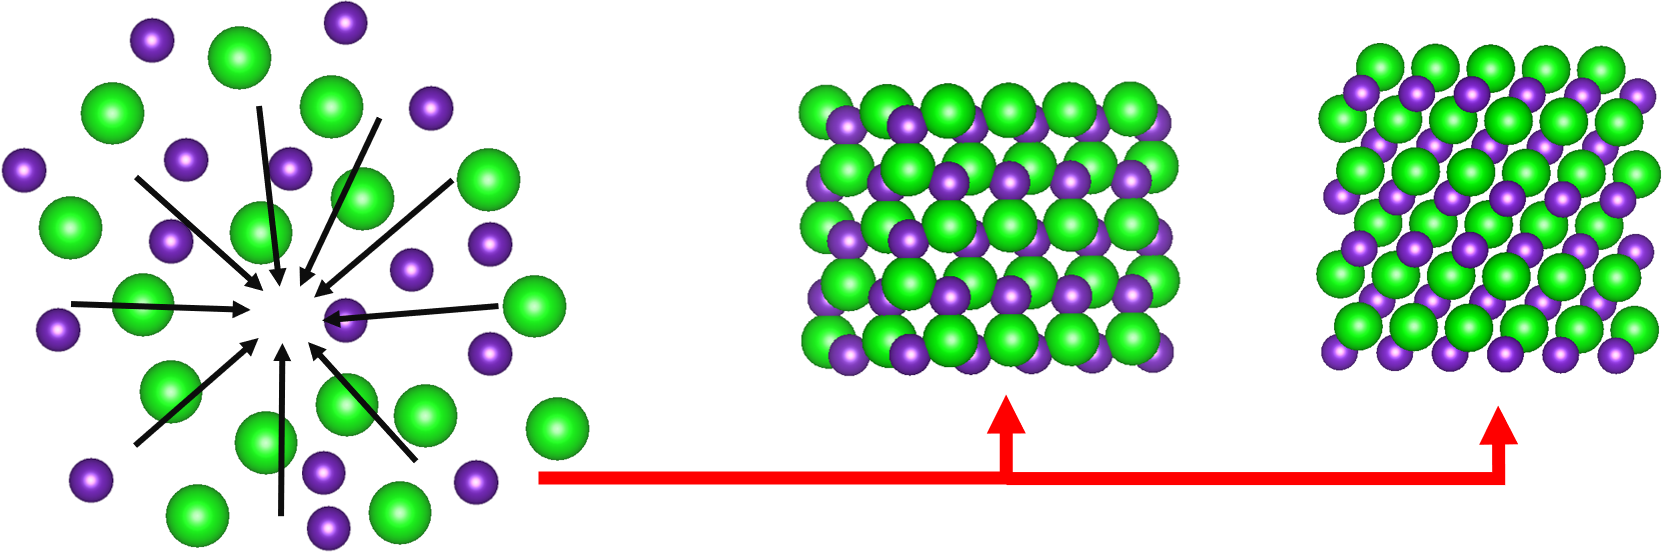
\includegraphics[trim={0cm 0cm 0cm 0cm},clip,width=0.45\linewidth]{figures/Nucleation_Overview.png}
\hspace*{\fill}
}
\date{April 29, 2019}

\sisetup{detect-weight=true, detect-family=true} % Allow bold SI units
\beamertemplatenavigationsymbolsempty % Remove navigation bar

\newcommand{\insertcurrentcitation}{}
\newcommand{\currentcitation}[1]{
	\renewcommand{\insertcurrentcitation}{#1}
} %Defining current citation for bottom left corner

\setbeamertemplate{footline}
{
  \leavevmode%
  \hbox{%
  \begin{beamercolorbox}[wd=.88\paperwidth,ht=2.25ex,dp=1ex,center]{author in head/foot}%
    \usebeamerfont{author in head/foot}\insertcurrentcitation
  \end{beamercolorbox}%
  %\begin{beamercolorbox}[wd=.25\paperwidth,ht=2.25ex,dp=1ex,center]{title in head/foot}%
  %  \usebeamerfont{title in head/foot}\insertshorttitle
  %\end{beamercolorbox}%
  \begin{beamercolorbox}[wd=.12\paperwidth,ht=2.25ex,dp=1ex,center]{date in head/foot}%
    \insertframenumber{} / \inserttotalframenumber\hspace*{1ex}
  \end{beamercolorbox}}%
  \vskip0pt%
}

\newcommand{\bb}[1]{\textcolor{red}{\textbf{#1}}}

\newcommand{\backupbegin}{
   \newcounter{finalframe}
   \setcounter{finalframe}{\value{framenumber}}
}
\newcommand{\backupend}{
   \setcounter{framenumber}{\value{finalframe}}
}


% Define Calorie
\DeclareSIUnit[number-unit-product = {\,}]
\cal{cal}
\DeclareSIUnit\kcal{\kilo\cal}


\begin{document}

%% title frame
\section[Introduction]{Introduction}
\begin{frame}
	\titlepage
\end{frame}


%% TOC
\subsection{Overview}
\begin{frame}
 \frametitle{Overview}
	\tableofcontents
\end{frame}

\subsection{What is Molecular Dynamics?}

\currentcitation{}
\begin{frame}
	\frametitle{What is Molecular Dynamics?}
	\begin{multicols}{2}
		\begin{center}
			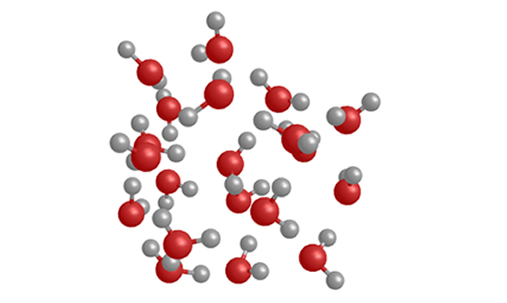
\includegraphics[trim={0.8cm 0cm 1cm 0cm},clip,width=0.42\textwidth]{figures/MD_Example.jpg}
		\end{center}
	\begin{itemize}
	\item Molecular Dynamics (MD) is a powerful \bb{computational method}.
	\pause
	\item Acts as a virtual microscope for \bb{model systems}.
	\pause
	\item \bb{Classical MD}: forces are calculated from pre-determined potential energy surface
		\begin{itemize}
			\item $ \vec{F}_{i}(t,\vec{r}_{i}) = -\vec{\nabla} u_{i}(t,\vec{r}_{i})$
			\item Time is discretized. \mbox{(1 - 10 $\SI{}{\femto\second}$)}
			\item Length Scales: up to \mbox{$10^{7}$ particles.} 
			\item Time Scales: up to $\SI{1}{\micro\second}$.
		\end{itemize}
	\end{itemize}
	\end{multicols}
\end{frame}

\begin{frame}
\frametitle{Problems with Molecular Dynamics}
	\begin{itemize}
		\item Classical MD is \bb{not exact}. Sources of error:
		\begin{itemize}
			\item Classical equations of motion \& empirical potentials.
			\item Many-body interactions usually approximated by \bb{effective two-body potentials}.
			\begin{equation}
				U = \sum_{i=1}\sum_{j>i} u_{ij} + \sum_{i=1}\sum_{j>i} \sum_{k>j} u_{ijk} + \ldots \approx \sum_{i=1} \sum_{j>i} u^{eff}_{ij}
			\end{equation}
			\item Finite-size/cutoff effects.
		\end{itemize}
		\pause
		\item Approximations make MD computationally efficient.
		\item Allow us to explore larger systems/longer times than \mbox{\bb{ab initio MD}.}
		\item Models are fit to specific properties, and not strictly \bb{transferable}, but often assumed to be.
	\end{itemize}
\end{frame}

\currentcitation{\cite{Karthika2016}}
\subsection{Classical Nucleation Theory}
\begin{frame}
\frametitle{Classical Nucleation Theory}
Want to improve our understanding of \bb{nucleation theory}.\\
Currently: \bb{Classical nucleation theory} (CNT)
	\begin{equation}
	\Delta G (r) = \frac {4 \pi r ^ { 3 } } { 3  }\rho \Delta g + 4 \pi r^{ 2 } \sigma
	\end{equation}
	\pause
\begin{center}
	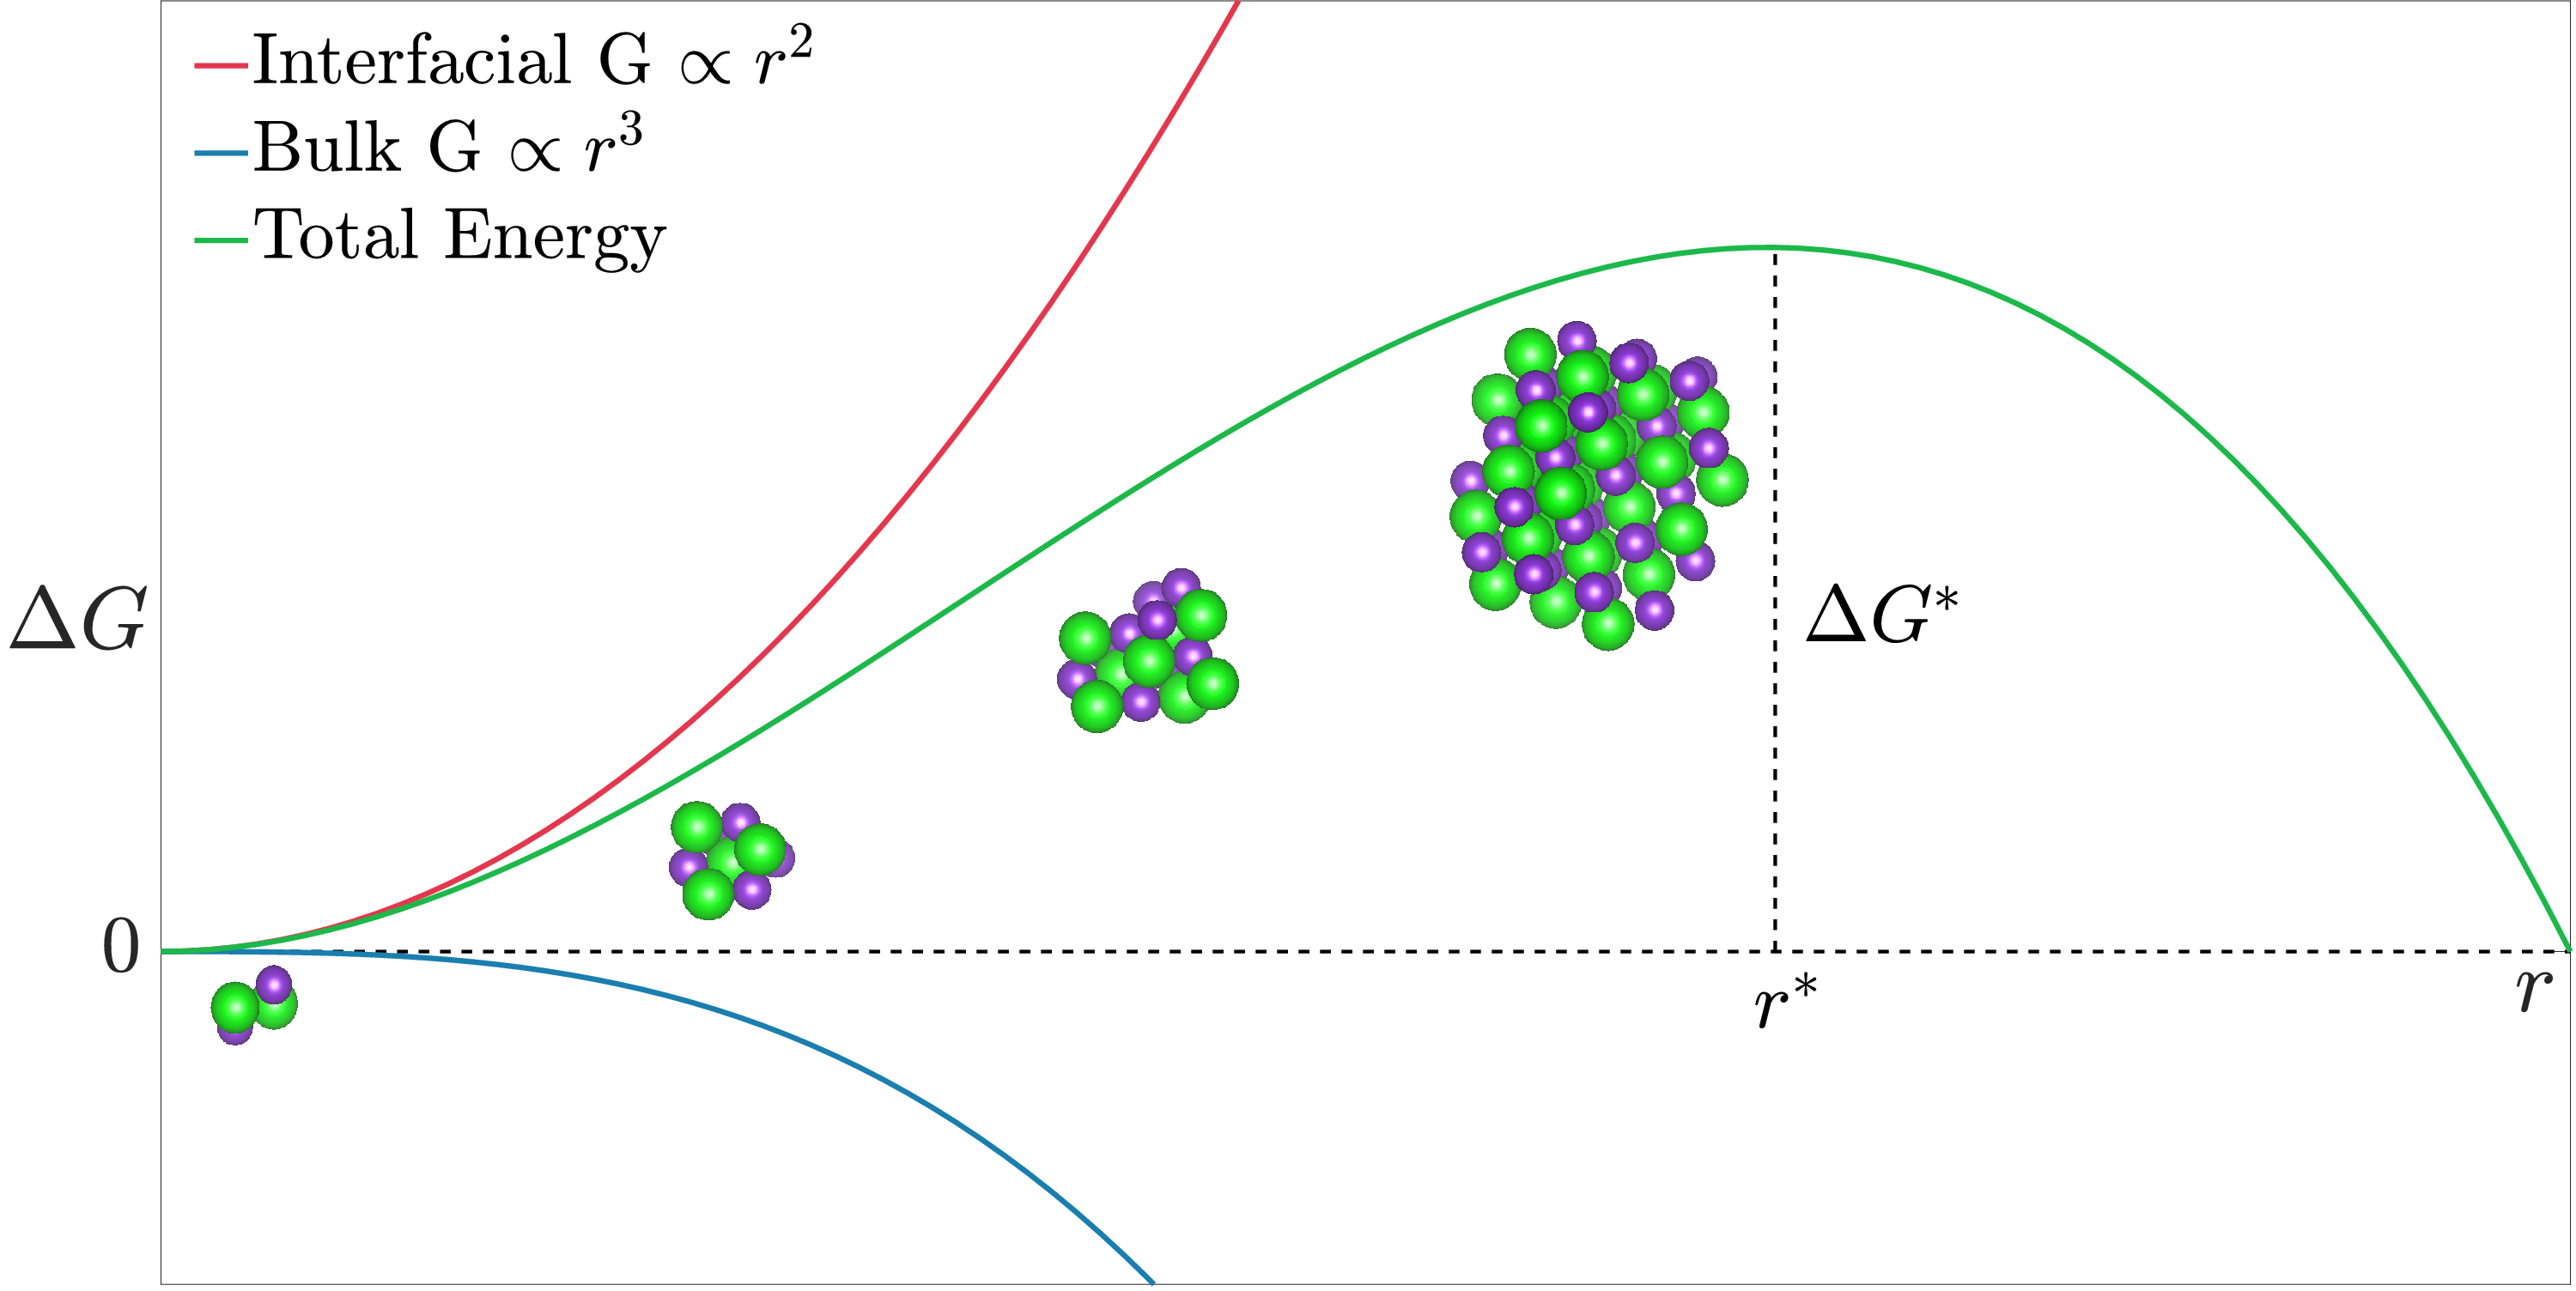
\includegraphics[trim={0cm 0cm 0cm 0cm},clip,width=0.85\textwidth]{figures/CNT.png}
\end{center}
\end{frame}


\subsection{Our Goal and Questions}
\begin{frame}
\frametitle{Our Goal}
\begin{itemize}
	\item Assumptions of CNT:
	\begin{itemize}
		\item Formation of \bb{perfectly spherical clusters}.
		\item Nucleation involves a \bb{single free energy barrier}.
		\item The interior/surface interactions of nuclei are equivalent to bulk phase interactions.
	\end{itemize}
	\item Despite these assumptions, CNT is a useful approximation. 
\end{itemize}
		\begin{center}
			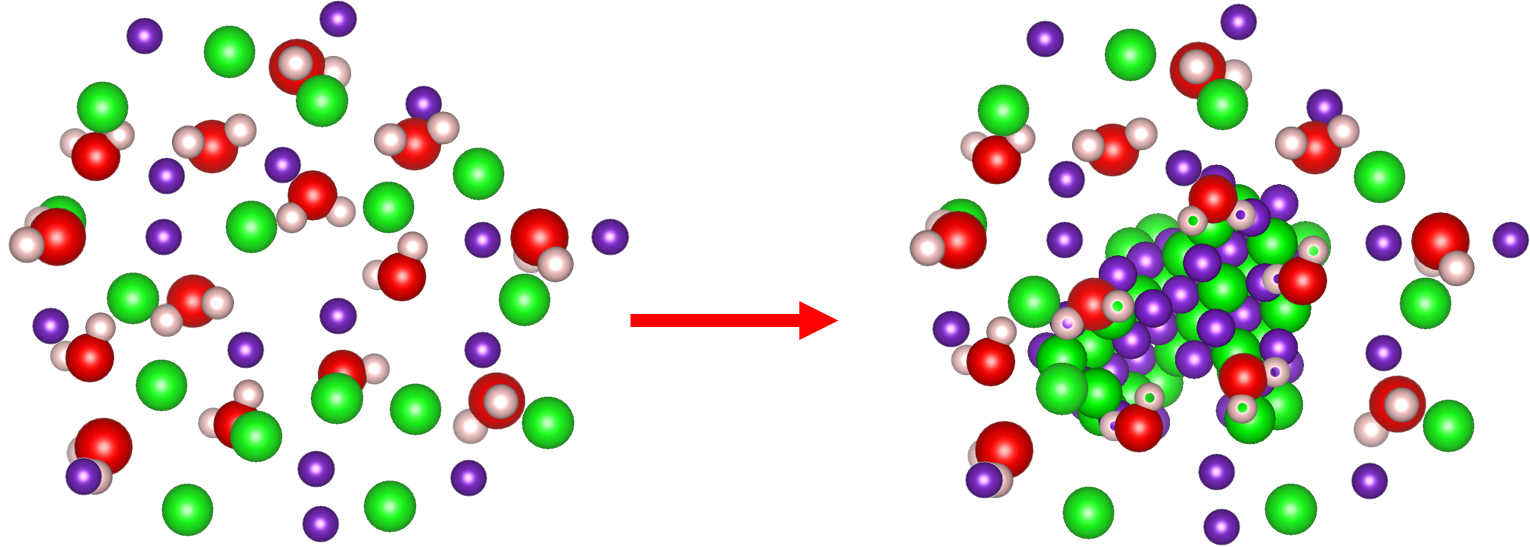
\includegraphics[trim={0cm 0cm 0cm 0cm},clip,width=0.8\textwidth]{figures/Nucleation.png}
		\end{center}
\end{frame}

\currentcitation{\cite{Lanaro2018}}
\begin{frame}
\frametitle{Main Questions}
	\textbf{I am interested in the cases where} \bb{CNT is deficient}. 
\begin{itemize}
	\item The lithium halides present a \bb{simple case study}.
	\pause
	\item Recent work shows that strong ion hydration may pose an activation barrier for nucleation.
	\begin{itemize}
		\item Is this barrier larger than the CNT barrier?
	\end{itemize}
	\pause
	\item Structural arrangement (or \bb{``crystallinity''}) of nuclei appears to play a critical role in nucleation.
	\begin{itemize}
		\item Mechanism/theoretical basis not well understood.
	\end{itemize}
	\pause
	\item In simulations, LiF does not nucleate at 300 K but does at 500 K. Why?
\end{itemize}
\end{frame}

\currentcitation{\cite{Lanaro2017}}
\begin{frame}
\frametitle{A big problem}

\textbf{Problem}: The available models \bb{usually fail to reproduce the correct crystal structures} of LiX in simulation!
\begin{itemize}
	\item Additionally, \bb{LiF solubility at 300 K is $\sim 10\times$ too soluble}.
	\item Two available models: \bb{Tosi-Fumi (TF)} and \bb{Joung-Cheatham (JC)}.
\end{itemize}
\begin{center}
	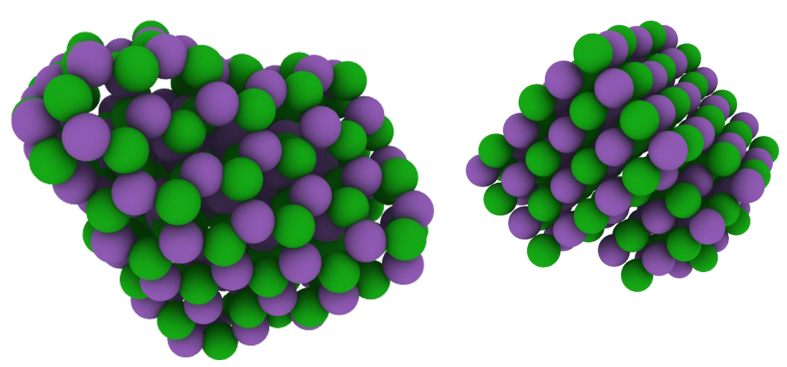
\includegraphics[trim={0cm 0cm 0cm 0cm},clip,width=0.65\textwidth]{figures/Nucleated_Clusters.png}
\end{center}
\bb{TF:} Fails for all lithium halides.\\ \bb{JC:} Fails for LiBr and LiI only (with SPC/E water).
\end{frame}

\begin{frame}
\frametitle{A big problem}
\begin{columns}
	\begin{column}{0.52\textwidth}
		JC Model:
		{\scriptsize
		\begin{align}
			u_{ij} (r_{ij}) = \frac{1}{4 \pi \varepsilon_{0}}\frac{q_{i} q_{j} }{r_{ij}} + 4 \epsilon_{ij} \bigg[ \big(\frac{\sigma_{ij}}{r_{ij}} \big)^{12} - \big(\frac{\sigma_{ij}}{r_{ij}} \big)^{6} \bigg]
		\end{align}}
		\begin{itemize}
			\item Coulombic Interaction + Lennard-Jones
			\item Fit to solvation free energies, RDF's, and lattice parameters, among others.
			\item Assumed \bb{rocksalt structure!}
		\end{itemize}
	\end{column}
\pause
	\begin{column}{0.52\textwidth}
		TF Model:
		{\scriptsize
		\begin{align}
		u_{ij} (r_{ij}) = \frac{1}{4 \pi \varepsilon_{0}}\frac{q_{i} q_{j} }{r_{ij}} + B_{ij} e^{-\alpha_{ij}r_{ij}}- \frac{C_{ij}}{r_{ij}^{6}} - \frac{D_{ij}}{r_{ij}^{8}}
		\end{align}}
		\begin{itemize}
			\item Coulombic Interaction + Exponential repulsion + dispersion.
			\item Fit to equation of state and derivatives, lattice energy, and lattice parameters.
			\item Assumed \bb{rocksalt structure!}
		\end{itemize}
	\end{column}
\end{columns}
\end{frame}

\currentcitation{}

\section{My Research}
\subsection{Solution: Improve the models!}
\begin{frame}
\frametitle{Goals of a model System}	
	\begin{enumerate}
		\item Correct ground state \bb{crystal structure}: Rocksalt.
		\item Correct \bb{solubility in water}.
		\pause
		Less importantly:
		\item Correct experimental \bb{lattice parameters} at 300 K.
		\item Correct experimental \bb{lattice energy}.
	\end{enumerate}
\pause
Points 3 and 4 are approximately true for JC and TF; points 1 and 2 not!
\begin{alertblock}{Side Note}
	Reported experimental lattice energies were inaccurate (improved). Experimental solubilities/lattice parameters are very accurate.
\end{alertblock}
\end{frame}

\subsection{Ab Initio Calculation Details}


\currentcitation{\cite{Peintinger2013}}
\begin{frame}
\frametitle{Overview}
\textbf{Our calculations were performed using} \bb{CRYSTAL17}.\\ 
This is a solid state HF/DFT \textit{ab initio} code which uses Gaussian basis functions.
\pause
\begin{itemize}
	\item Crystal atomic orbitals are expanded periodically as \bb{Bloch functions}.
	\item Recently (2013/2018) released \bb{``pob-TZVP''} basis set is highest quality available for periodic calculations.
	\item Based on \bb{``def2‐TZVP''} basis sets developed for molecules.
	\item Optimized variationally for solid state. Training sets included \bb{LiX in rocksalt structure}.
	\item Our study tested wide range of DFT exchange-correlation (XC) functionals.
\end{itemize}
\end{frame}

\begin{frame}
\frametitle{Most Important Choice: Basis Set}
\begin{alertblock}{From Experience:}
	In solid state DFT, choice of Basis set is extremely important.
\end{alertblock}
	\begin{center}
	\includegraphics[trim={0cm 0cm 0cm 0cm},clip,width=\textwidth]{\figfile/Basis_Set_Dependence.eps}
	\end{center}
\end{frame}

\currentcitation{}
\begin{frame}
\frametitle{Less Important Choice: XC Functional}
\begin{alertblock}{From Experience:}
	For solid state DFT, the XC is less important.
\end{alertblock}
\begin{center}
	\includegraphics[trim={0cm 0cm 0cm 0cm},clip,width=\textwidth]{\figfile/XC_Dependence_DeltaE_NoD3.eps}
\end{center}
\end{frame}

\begin{frame}
\frametitle{Less Important Choice: XC Functional}
How to choose the XC functional: comparison with experiment.
\begin{center}
	\includegraphics<1>[trim={0cm 0cm 0cm 0cm},clip,width=\textwidth]{\figfile/XC_Dependence_DeltaEExp.eps}
	\includegraphics<2>[trim={0cm 0cm 0cm 0cm},clip,width=\textwidth]{\figfile/XC_Dependence_DeltaAExp.eps}
\end{center}
\end{frame}

\subsection{Comparison of Potentials}
\begin{frame}
\frametitle{Comparison of Potentials: Crystal Potential}
\begin{center}
	\includegraphics[trim={0cm 0cm 0cm 0cm},clip,width=\textwidth]{\figfile/a_vs_E.eps}
\end{center}
\end{frame}


\subsection{Importance of Dispersion}

\begin{frame}
\frametitle{Importance of Dispersion: Ab initio methods}
\begin{center}
	\includegraphics[trim={0cm 0cm 0cm 0cm},clip,width=\textwidth]{\figfile/a_vs_Dispersion_Bar.eps}
\end{center}
\end{frame}

\currentcitation{}
\begin{frame}
\frametitle{Importance of Dispersion: Empirical models}
	What if we \bb{scale} the dispersion interaction in empirical models by a factor \bb{$\mathbf{S_{D}}$}?
	\only<1-1>{
	\begin{align}
	u^{JC}_{ij} &= \frac{1}{4 \pi \varepsilon_{0}}\frac{q_{i} q_{j} }{r} + 4 \epsilon \bigg[ \big(\frac{\sigma_{ij}}{r} \big)^{12} - {\color{red}\mathbf{S_{D}}}\big(\frac{\sigma_{ij}}{r} \big)^{6} \bigg]\\
	u^{TF}_{ij} &= \frac{1}{4 \pi \varepsilon_{0}}\frac{q_{i} q_{j} }{r} + B_{ij} e^{-\alpha_{ij}r} - {\color{red}\mathbf{S_{D}}}\bigg(\frac{C_{ij}}{r^{6}} + \frac{D_{ij}}{r^{8}}\bigg)
	\end{align}}
	\begin{center}
		\includegraphics<2>[trim={0cm 0cm 0cm 0cm},clip,width=\textwidth]{\figfile/EmpDisp_Dependence_DeltaE.eps}
	\end{center}
\end{frame}

\begin{frame}
\frametitle{Summary}
\textbf{In my research so far, we have found:}
\begin{itemize}
	\item TF empirical model favours wurtzite in all cases, yet its PES matches best with ab initio calculations.
	\item JC empirical model favours rocksalt in LiF and LiCl, but has incorrect energies at high pressure.
	\item Ab initio calculations show that wurtzite and rocksalt are very close in energy.
	\item The dispersion interaction is weak but favours rocksalt in both DFT calculations and empirical models.
\end{itemize}
\end{frame}


\section{Future Work}	
\subsection{Nucleation Mechanism of LiX Salts}
\begin{frame}
\frametitle{Future Work: Nucleation Mechanism of LiX}
With a working model for the lithium halides, can explore \bb{non-classical nucleation mechanisms}.\\
Unanswered Questions:
\begin{itemize}
	\item Why does dispersion favour rocksalt?
	\item Is there a single free energy barrier to LiX nucleation?
	\item How does ion size affect the nucleation mechanism?
	\item Why does LiF solubility decrease at higher temperatures?
\end{itemize}
\end{frame}

\subsection{Acknowledgments}
\begin{frame}
\frametitle{Acknowledgments}
	\textbf{Thank you to the following for making this research possible:}\\
\begin{center}
	\Large{Prof. Gren Patey, Supervisor}\\
\end{center}
\begin{columns}
	\begin{column}{0.5\textwidth}
	
\includegraphics[trim={0cm 0cm 0cm 0cm},clip,width=\textwidth]{figures/ComputeCanada_logo.png}
	\end{column}
	\begin{column}{0.5\textwidth}
	
\includegraphics[trim={0cm 0cm 0cm 0cm},clip,width=\textwidth]{figures/NSERC.png}
	\end{column}
\end{columns}
\begin{center}

\includegraphics[trim={0cm 0cm 0cm 0cm},clip,width=0.7\textwidth]{figures/UBC_Chemlogo.eps}
\end{center}
\end{frame}


%---------------------EXTRA SLIDES----------------------------------%
\backupbegin
\currentcitation{}
\section{}
\subsection{}
\begin{noheadline}
	
\begin{frame}
\frametitle{Comparison of Potentials: Pair Potential}
\begin{center}
	\includegraphics[trim={0cm 0cm 0cm 0cm},clip,width=\textwidth]{\figfile/Pair_Potentials.eps}
\end{center}
\end{frame}

\begin{frame}
\frametitle{JC With Different Water Models}
\begin{table}[]
	{\tiny
	\begin{tabular}{l|lllllll}
		Species & Model & Favoured & Rocksalt $E_{L}$ & Wurtzite $E_{L}$ & $\Delta E_{L}$ & $a_{Rock}$ & $a_{Wurtz}$ \\ \hline
		\multirow{5}{*}{LiF} & Experimental & Rocksalt & -1054(1) &  &  & 4.02620(5) &  \\
		& JC (SPC/E) & Rocksalt & -1052.59 & -1030.51 & -22.08 & 4.29 & 3.35 \\
		& JC (TIP3P) & Rocksalt & -1093.77 & -1073.72 & -20.05 & 4.09 & 3.19 \\
		& JC (TIP4P$_{EW}$) & Rocksalt & -1059.52 & -1041.3 & -18.22 & 4.23 & 3.3 \\
		& TF & Wurtzite & -1043.11 & -1051.97 & 8.86 & 4.01 & 2.99 \\ \hline
		\multirow{5}{*}{LiCl} & Experimental & Rocksalt & -865(2) &  &  & 5.13988(4) &  \\
		& JC (SPC/E) & Rocksalt & -870.32 & -863.58 & -6.74 & 5.2 & 4.01 \\
		& JC (TIP3P) & Wurtzite & -891.53 & -899.88 & 8.35 & 5.08 & 3.84 \\
		& JC (TIP4P$_{EW}$) & Wurtzite & -877.65 & -883.34 & 5.69 & 5.14 & 3.91 \\
		& TF & Wurtzite & -844.73 & -846.9 & 2.17 & 5.08 & 3.81 \\ \hline
		\multirow{5}{*}{LiBr} & Experimental & Rocksalt & -821(2) &  &  & 5.501(6) &  \\
		& JC (SPC/E) & Wurtzite & -826.03 & -826.78 & 0.75 & 5.51 & 4.21 \\
		& JC (TIP3P) & Wurtzite & -836.91 & -853.04 & 16.13 & 5.43 & 4.07 \\
		& JC (TIP4P$_{EW}$) & Wurtzite & -826.72 & -842.58 & 15.86 & 5.49 & 4.12 \\
		& TF & Wurtzite & -795.68 & -796.72 & 1.04 & 5.44 & 4.08 \\ \hline
		\multirow{5}{*}{LiI} & Experimental & Rocksalt & -764(1) &  &  & 6.012(7) &  \\
		& JC (SPC/E) & Wurtzite & -761.78 & -770.2 & 8.42 & 6 & 4.54 \\
		& JC (TIP3P) & Wurtzite & -768.97 & -790.37 & 21.4 & 5.91 & 4.4 \\
		& JC (TIP4P$_{EW}$) & Wurtzite & -760.92 & -782.98 & 22.06 & 5.98 & 4.45 \\
		& TF & Wurtzite & -720.06 & -729.49 & 9.43 & 5.93 & 4.39
	\end{tabular}
	}
\end{table}
\end{frame}

% Born-Oppenheimer Approximation
\begin{frame}
\frametitle{Born-Oppenheimer Approximation}
{\tiny
\begin{equation*}
\Ham \Psi = E \Psi
\end{equation*}
where
\begin{equation*}
\Ham = -\frac{1}{2}\sum_{i=1}^{N} \nabla_{i}^{2} -\frac{1}{2} \sum_{A=1}^{M} \frac{1}{M_{A}} \nabla_{A}^{2} + 
\sum_{i=1}^{N} \sum_{j>i}^{N} \frac{1}{r_{ij}} + \sum_{A=1}^{M} \sum_{B>A}^{M} \frac{Z_{A} Z_{B}}{R_{AB}} -
\sum_{i=1}^{N} \sum_{A = 1}^{M} \frac{Z_{A}}{r_{iA}}.
\end{equation*}
Assume
\begin{equation*}
\Psi(\vec{r}_{1}, \ldots , \vec{r}_{N}, \vec{R}_{1}\ldots , \vec{R}_{M}) = \Psi_{elec}(\vec{r}_{1}, \ldots , \vec{r}_{N}; \vec{R}_{1}\ldots , \vec{R}_{M}) \Psi_{nucl}(\vec{R}_{1},\ldots , \vec{R}_{M}).
\end{equation*}
\begin{align*}
\Ham \Psi_{elec} \Psi_{nucl} &= -\frac{1}{2}\sum_{i=1}^{N} \Psi_{nucl} \bigg( \nabla^{2}_{i} \Psi_{elec} \bigg) -\frac{1}{2} \sum_{A=1}^{M} \frac{1}{M_{A}} \nabla_{A}^{2} \bigg( \Psi_{elec} \Psi_{nucl} \bigg) + \bigg( \sum_{i=1}^{N} \sum_{j>i}^{N} \frac{1}{r_{ij}} \bigg) \Psi_{elec} \Psi_{nucl}\\ &+ \bigg( \sum_{A=1}^{M} \sum_{B>A}^{M} \frac{Z_{A} Z_{B}}{R_{AB}} \bigg) \Psi_{elec} \Psi_{nucl} - \bigg( \sum_{i=1}^{N} \sum_{A = 1}^{M} \frac{Z_{A}}{r_{iA}} \bigg) \Psi_{elec} \Psi_{nucl}\\
&=\bigg( \underbrace{\bigg( -\frac{1}{2}\sum_{i=1}^{N} \nabla^{2}_{i} + \sum_{i=1}^{N} \sum_{j>i}^{N} \frac{1}{r_{ij}} - \sum_{i=1}^{N} \sum_{A = 1}^{M} \frac{Z_{A}}{r_{iA}} \bigg)}_\text{Electronic Hamiltonian} \Psi_{elec} \bigg) \Psi_{nucl} + \bigg( \sum_{A=1}^{M} \sum_{B>A}^{M} \frac{Z_{A} Z_{B}}{R_{AB}} \bigg) \Psi_{elec} \Psi_{nucl}\\
&-\frac{1}{2} \sum_{A=1}^{M} \frac{1}{M_{A}} \bigg( \underbrace{\big( \nabla_{A}^{2} \Psi_{elec} \big)}_\text{Neglect} \Psi_{nucl} + \underbrace{\big(\nabla_{A}^{2} \Psi_{nucl} \big)}_\text{Keep} \Psi_{elec} + 2 \underbrace{\big(\nabla_{A} \Psi_{elec} \big)\big( \nabla_{A} \Psi_{nucl} \big)}_\text{Neglect} \bigg)
\end{align*}
}
\end{frame}

\begin{frame}
\frametitle{Born-Oppenheimer Approximation}
{\tiny
Neglecting the indicated terms on the previous slide yields
	\begin{align*}
	\Ham \Psi_{elec} \Psi_{nucl} &\approx \bigg( \underbrace{\bigg( -\frac{1}{2}\sum_{i=1}^{N} \nabla^{2}_{i} + \sum_{i=1}^{N} \sum_{j>i}^{N} \frac{1}{r_{ij}} - \sum_{i=1}^{N} \sum_{A = 1}^{M} \frac{Z_{A}}{r_{iA}} \bigg)}_{\varepsilon_{elec}} \Psi_{elec} \bigg) \Psi_{nucl} + \bigg( \sum_{A=1}^{M} \sum_{B>A}^{M} \frac{Z_{A} Z_{B}}{R_{AB}} \bigg) \Psi_{elec} \Psi_{nucl}\\
	&-\frac{1}{2} \sum_{A=1}^{M} \frac{1}{M_{A}} \big(\nabla_{A}^{2} \Psi_{nucl} \big) \Psi_{elec} = E \Psi_{elec} \Psi_{nucl} 
	\end{align*}
	The electronic problem is solved separately, with the nuclear degrees of freedom treated parametrically to yield $\varepsilon_{elec}$. The nuclear problem can then be solved separately as
	\begin{align*}
	\bigg( -\frac{1}{2} \sum_{A=1}^{M} \frac{1}{M_{A}} \nabla_{A}^{2} + \underbrace{\sum_{A=1}^{M} \sum_{B>A}^{M} \frac{Z_{A} Z_{B}}{R_{AB}} + \varepsilon_{elec}}_\text{P.E. landscape for nuclear motion} \bigg) \Psi_{nucl} = E \Psi_{nucl}
	\end{align*}
}
\end{frame}

\begin{frame}
\frametitle{Born-Oppenheimer Approximation}
{\tiny
	Neglecting the indicated terms on the previous slide yields
	\begin{align*}
	\Ham \Psi_{elec} \Psi_{nucl} &\approx \bigg( \underbrace{\bigg( -\frac{1}{2}\sum_{i=1}^{N} \nabla^{2}_{i} + \sum_{i=1}^{N} \sum_{j>i}^{N} \frac{1}{r_{ij}} - \sum_{i=1}^{N} \sum_{A = 1}^{M} \frac{Z_{A}}{r_{iA}} \bigg)}_{\varepsilon_{elec}} \Psi_{elec} \bigg) \Psi_{nucl} + \bigg( \sum_{A=1}^{M} \sum_{B>A}^{M} \frac{Z_{A} Z_{B}}{R_{AB}} \bigg) \Psi_{elec} \Psi_{nucl}\\
	&-\frac{1}{2} \sum_{A=1}^{M} \frac{1}{M_{A}} \big(\nabla_{A}^{2} \Psi_{nucl} \big) \Psi_{elec} = E \Psi_{elec} \Psi_{nucl} 
	\end{align*}
	The electronic problem is solved separately, with the nuclear degrees of freedom treated parametrically to yield $\varepsilon_{elec}$. The nuclear problem can then be solved separately as
	\begin{align*}
	\bigg( -\frac{1}{2} \sum_{A=1}^{M} \frac{1}{M_{A}} \nabla_{A}^{2} + \underbrace{\sum_{A=1}^{M} \sum_{B>A}^{M} \frac{Z_{A} Z_{B}}{R_{AB}} + \varepsilon_{elec}}_\text{P.E. landscape for nuclear motion} \bigg) \Psi_{nucl} = E \Psi_{nucl}.
	\end{align*}
	If one wishes to do MD in this way, the electronic problem must be re-solved for each time step.
}
\end{frame}


\begin{frame}
\frametitle{DFT: Kohn-Sham Method}
{\tiny
	The Kohn-Sham method for the ground electronic state. Start with the electronic problem
	\begin{align*}
	\Ham_{elec} \Psi_{i} = E_{i} \Psi{i}
	\end{align*}
	where $\Psi{i}$ is the many-electron wavefunction. The Hamiltonian is
	\begin{align*}
	\Ham_{elec} = -\frac{1}{2}\sum_{i=1}^{N} \nabla^{2}_{i} + \sum_{i=1}^{N} \sum_{j>i}^{N} \frac{1}{r_{ij}} - \sum_{i=1}^{N} \underbrace{\bigg( \sum_{A = 1}^{M} \frac{Z_{A}}{r_{iA}} \bigg)}_{V(\vec{r}_{i})}.
	\end{align*}
	In KS DFT this problem is converted into
	\begin{align*}
	\Ham_{eff} \psi_{i} = \varepsilon_{i} \psi_{i}
	\end{align*}
	where $\psi_{i}$ are one-electron functions and
	\begin{align*}
	\Ham_{eff} = -\frac{1}{2} \nabla^{2} + V_{eff}.
	\end{align*}
	$V_{eff}$ is the mean-field effective potential created by the nuclei and other electrons acting on the electron of interest. It contains the external potential $V(\vec{r}_{i})$, the electron-electron Coulomb potential, the exchange potential, and the correlation potential.\\
	The premise of KS DFT: one can work with electron density $\rho(\vec{r})$ instead of the many-electron wavefunction $\Psi_{i} (\vec{r}_{1}, \vec{r}_{2},\ldots,\vec{r}_{N} )$. This is shown in the theorems of Kohn and Sham.
}
\end{frame}

\begin{frame}
\frametitle{DFT: Kohn-Sham Method: Theorem 1}
{\tiny
	\textbf{Theorem 1}: the external potential, $V(\vec{r})$, acting on a fully-interacting system of $N$ electrons in its ground state is determined (within an additive constant) by the electron density.\\
	\textbf{Proof}: by contradiction.\\
	Imagine you have two different external potentials, $V(\vec{r})$ and $V^{\prime}(\vec{r})$, differing by more than a constant and leading to the same electron density $\rho(\vec{r})$ in the ground state.
	\begin{align*}
	V(\vec{r}) &\rightarrow \Ham\\
	V^{\prime}(\vec{r}) &\rightarrow \Ham^{\prime}.
	\end{align*}
	These Hamiltonians have the same kinetic and electron-electron terms, but differ in their nuclear-electron term. Applying these two the electronic Schr\"{o}dinger equation leads to
	\begin{align*}
	\Ham \Psi_{0} &= E_{0} \Psi_{0} \\
	\Ham^{\prime} \Psi^{\prime}_{0} &= E^{\prime}_{0} \Psi^{\prime}_{0}.
	\end{align*}
	The variational theorem tells us that $\bra{\Psi^{\prime}_{0}} \Ham \ket{\Psi^{\prime}_{0}} > E_{0}$ and $\bra{\Psi_{0}} \Ham^{\prime} \ket{\Psi_{0}} > E_{0}$. Writing this explicitly,
	\begin{align*}
	\bra{\Psi^{\prime}_{0}} \Ham \ket{\Psi^{\prime}_{0}} &= \int \Psi^{\prime *}_{0} (\rall) \bigg(\frac{-1}{2}\sum_{i=1}^{N} \nabla_{i}^{2} \bigg) \Psi^{\prime}_{0} (\rall) \drall\\ 
	&+ \int \Psi^{\prime *}_{0} (\rall) \bigg(\sum_{i=1}^{N} \sum_{j>i}^{N} \frac{1}{r_{ij}}\bigg) \Psi^{\prime}_{0} (\rall) \drall\\
	&+ \int \Psi^{\prime *}_{0} (\rall) \bigg(\sum_{i=1}^{N} V(\vri)\bigg) \Psi^{\prime}_{0} (\rall) \drall.
	\end{align*}
}
\end{frame}

\begin{frame}
\frametitle{DFT: Kohn-Sham Method: Theorem 1}
{\tiny
	We can also write this as
	\begin{align*}
	\bra{\Psi^{\prime}_{0}} \Ham \ket{\Psi^{\prime}_{0}} &= T^{\prime} + E_{ee}^{\prime} + \int \Psi^{\prime *}_{0} (\rall) \bigg(\sum_{i=1}^{N} \int V(\vec{r}) \delta(\vec{r} - \vri ) d\vec{r} \bigg) \Psi^{\prime}_{0} (\rall) \drall,
	\end{align*}
	where the inner integral collapses due to the delta function $\delta(\vec{r} - \vri )$. Rearranging,
	\begin{align*}
	\bra{\Psi^{\prime}_{0}} \Ham \ket{\Psi^{\prime}_{0}} &= T^{\prime} + E_{ee}^{\prime} + 
	\int V(\vec{r}) d\vec{r} \underbrace{\int \Psi^{\prime *}_{0} (\rall) \bigg(\sum_{i=1}^{N} \delta(\vec{r} - \vri )  \bigg) \Psi^{\prime}_{0} (\rall) \drall}_\text{Electron Density}\\
	&= T^{\prime} + E_{ee}^{\prime} + \int V(\vec{r}) \rho(\vec{r}) d\vec{r} > E_{0} \quad \text{(assumption)}.
	\end{align*}
	Now we also have 
	\begin{align*}
	\bra{\Psi_{0}} \Ham^{\prime} \ket{\Psi_{0}} = \ldots = T + E_{ee} + \int V^{\prime}(\vec{r}) \rho(\vec{r}) d\vec{r} > E^{\prime}_{0}.
	\end{align*}
	We can also write
	\begin{align*}
	E_{0} < \bra{\Psi^{\prime}_{0}} \Ham \ket{\Psi^{\prime}_{0}} = \bra{\Psi^{\prime}_{0}} \Ham - \Ham^{\prime} \ket{\Psi^{\prime}_{0}} \bra{\Psi^{\prime}_{0}} \Ham^{\prime} \ket{\Psi^{\prime}_{0}} = \int \big( V(\vec{r}) - V^{\prime}(\vec{r}) \big) \rho(\vec{r}) d\vec{r} + E^{\prime}_{0}.
	\end{align*}
}
\end{frame}

\begin{frame}
\frametitle{DFT: Kohn-Sham Method: Theorem 1}
{\tiny
	So far we have
	\begin{align}
	E_{0} < E^{\prime}_{0} + \int \big( V(\vec{r}) - V^{\prime}(\vec{r}) \big) \rho(\vec{r}) d\vec{r},
	\label{eq1a}
	\end{align}
	but we can also write
	\begin{align}
	\nonumber E^{\prime}_{0} < \bra{\Psi_{0}} \Ham^{\prime} \ket{\Psi_{0}} = \int \big( V^{\prime}(\vec{r}) - V(\vec{r}) \big) \rho(\vec{r}) d\vec{r} + E_{0}\\
	E^{\prime}_{0} < E_{0} - \int \big( V(\vec{r}) - V^{\prime}(\vec{r}) \big) \rho(\vec{r}) d\vec{r}
	\label{eq2a}
	\end{align}
	Now add equations~\ref{eq1a} and~\ref{eq2a} to get
	\begin{align*}
	E_{0} + E^{\prime}_{0} < E_{0} + E^{\prime}_{0}
	\end{align*}
	which is a contradiction. Hence our original assumption that two different external potentials can lead to the same electron density is wrong. This means that $\rhovr$ uniquely determines $V(\vec{r})$ which uniquely determines the one electron Hamiltonian $\Ham$ which uniquely determines the ground state energy and wavefunction. The problem of $3N$ variables can be rewritten as a problem of 3 variables.
}
\end{frame}


\begin{frame}
\frametitle{DFT: Kohn-Sham Method: Theorem 2}
{\tiny
	\textbf{Theorem 2}: The variation principle in terms of electron density.\\
	
	\textbf{Proof}: Assume $\rho(\vec{r})$ is the correct ground state density and $\rho^{\prime}(\vec{r})$ is a trial density. From theorem 1, we saw that the ground state energy can be written as a functional of the electron density
	\begin{align*}
	E_{0}[\rhovr] = \underbrace{T[\rhovr] + U_{ee} [\rhovr]}_{F_{HK}[\rhovr]} + \int V(\vec{r}) \rhovr d\vec{r}.
	\end{align*}
	The arbitrary trial density $\rho^{\prime}(\vec{r})$ uniquely defines a wavefunction $\Psi_{0}^{\prime}$, but we know from the variational principle that
	\begin{align*}
	\bra{\Psi^{\prime}_{0}} \Ham \ket{\Psi^{\prime}_{0}} \geq E_{0}.
	\end{align*}
	But theorem 1 showed us that
	\begin{align*}
	\bra{\Psi^{\prime}_{0}} \Ham \ket{\Psi^{\prime}_{0}} = F_{HK}[\rhovr] + \int V(\vec{r}) \rhovr^{\prime} d\vec{r}.
	\end{align*}
	Hence
	\begin{align*}
	F_{HK}[\rhovr] + \int V(\vec{r}) \rhovr^{\prime} d\vec{r} \geq E_{0}.
	\end{align*}
	From theorem 1, the equality is true only if $\rho^{\prime}(\vec{r}) = \rho(\vec{r})$.
}
\end{frame}

\begin{frame}
\frametitle{DFT: Kohn-Sham Method}
{\tiny
	From theorems 1 and 2, we know that the external potential is fully determined if the electron density is known. That means we can work with $\rhovr$ instead of the all electron wavefunction, i.e. 3 variables instead of $3N$.\\
	The Kohn-Sham method is to imagine a reference system of non-interacting electrons,
	\begin{align*}
	\Ham_{ref} = -\frac{1}{2}\sum_{i=1}^{N} \nabla^{2}_{i} + \sum_{i=1}^{N} V_{ref}(\vri),
	\end{align*}
	which would lead to the one-electron problem
	\begin{align*}
	\Ham_{ref}\psi_{i} = \varepsilon_{i}\psi_{i}.
	\end{align*}
	The key is to choose $V_{ref}(\vri)$ (the external potential of the reference system) such that the electron density of this reference system is equal to the electron density of the actual system of interest. This (after a fairly long derivation) leads to the Kohn-Sham equations
	\begin{align*}
	\Ham_{eff} = -\frac{1}{2} \nabla^{2} + V_{eff} (\vec{r})
	\end{align*}
	where
	\begin{align*}
	V_{eff} (\vec{r}) &= V (\vec{r}) + \int \frac{\rho (\vec{r}^{\prime})}{|\vec{r} - \vec{r}^{\prime} |} d\vec{r}^{\prime} + \frac{\delta E_{XC}[\rhovr]}{\delta \rhovr}\\
	\rhovr &= \sum_{i=1}^{N} \psi_{i}^{*}(\vec{r}) \psi_{i}(\vec{r}) 
	\end{align*}
	The one-electron orbitals are given by
	\begin{align*}
	\Ham_{eff}\psi_{i} = \varepsilon_{i}\psi_{i}.
	\end{align*}
}
\end{frame}

\begin{frame}
\frametitle{DFT: Kohn-Sham Method Summary}
{\tiny
	\textbf{The Kohn-Sham Method:}\\
	
	Begin with $N$ trial wavefunctions \{$\psi_{i}$\}
	\begin{align*}
	&1)\quad \rhovr = \sum_{i=1}^{N} \psi_{i}^{*}(\vec{r}) \psi_{i}(\vec{r})\\
	&2)\quad V_{eff} = V (\vec{r}) + \int \frac{\rho (\vec{r}^{\prime})}{|\vec{r} - \vec{r}^{\prime} |} d\vec{r}^{\prime} + \underbrace{\frac{\delta E_{XC}[\rhovr]}{\delta \rhovr}}_{V_{XC}[\rhovr]}\\
	&3)\quad \Ham_{eff} = -\frac{1}{2} \nabla^{2} + V_{eff} (\vec{r})\\
	&4)\quad \Ham_{eff}\psi_{i} = \varepsilon_{i}\psi_{i}
	\end{align*}
	Repeat steps 1-4 until energy is sufficiently converged between cycles. Once convergence is achieved, the total energy is calculated as a functional of the electron density:
	\begin{align*}
	E[\rhovr] = \sum_{i=1}^{N} \int \psi_{i}^{*}(\vec{r}) \big( -\frac{1}{2} \nabla^{2} \big) \psi_{i}(\vec{r}) d\vec{r} + \int V (\vec{r}) \rhovr d\vec{r} + \frac{1}{2} \int \frac{\rho(\vec{r}^{\prime})}{\vec{r} - \vec{r}^{\prime}} d\vec{r} + E_{XC}[\rhovr]
	\end{align*}
	or equivalently
	\begin{align*}
	E[\rhovr] = \sum_{i=1}^{N} \varepsilon_{i} - \frac{1}{2} \int \frac{\rho(\vec{r}^{\prime})\rhovr}{|\vec{r}^{\prime} - \vec{r}|} d\vec{r}^{\prime}d\vec{r} + E_{XC} [\rhovr] - \int \frac { \delta E _ { XC } [ \rhovr ] } { \delta \rhovr } \rhovr d \vec { r }.
	\end{align*}
}
\end{frame}



\begin{frame}
\frametitle{Ewald Summation}
The total interaction energy of a 3D periodic system of point charges is
\begin{equation*}
E = \frac { 1 } { 4 \pi \varepsilon _ { 0 } } \sum _ { \mathbf { n } } \frac{1}{2} \sum _ { i = 1 } ^ { N } \sideset{}{'}\sum _ { j = 1} ^ { N} \frac { q _ { i } q _ { j } } { \left| \mathbf { r } _ { i j } + \mathbf { n } \right| }
\end{equation*}
where $\mathbf{n} = n_1 \mathbf{a} + n_2 \mathbf{b} + n_3 \mathbf{c}$ are periodic, but this straightforward sum is only conditionally convergent, and converges slowly.\\
\vspace{1em}
Ewald summation converts this conditionally convergent sum in real space into two quickly and absolutely convergent sums: one in real space and one in reciprocal ($\mathbf{k}$) space.
\end{frame}

\begin{frame}
\frametitle{Ewald Summation}
Ewald summation relies on the fact that the charge distribution is \bb{periodic}. It takes a \bb{Fourier transform} of the long range interaction.
\begin{align*} 
	E & =  E ^ { S } + E ^ { L } - E ^ { \mathrm { self } } \\ &=  \frac { 1 } { 4 \pi \varepsilon _ { 0 } } \frac { 1 } { 2 } \sum _ { \mathbf { n } } \sum _ { i = 1 } ^ { N } \sideset{}{'}\sum _ { j = 1 } ^ { N } \frac { q _ { i } q _ { j } } { \left| \mathbf { r } _ { i } - \mathbf { r } _ { j } + \mathbf { n L } \right| } \operatorname { erfc } \left( \frac { \left| \mathbf { r } _ { i } - \mathbf { r } _ { j } + \mathbf { n } L \right| } { \sqrt { 2 } \sigma } \right) \\ & + \frac { 1 } { 2 V \varepsilon _ { 0 } } \sum _ { \mathbf { k } \neq \mathbf { 0 } } \frac { \mathrm { e } ^ { - \sigma ^ { 2 } k ^ { 2 } / 2 } } { k ^ { 2 } } | S ( \mathbf { k } ) | ^ { 2 } - \frac { 1 } { 4 \pi \varepsilon _ { 0 } } \frac { 1 } { \sqrt { 2 \pi } \sigma } \sum _ { i = 1 } ^ { N } q _ { i } ^ { 2 } 
\end{align*}
Self correction term corrects the long range summation, which includes the self interaction in order to maintain the \bb{periodicity of the interaction.}
\end{frame}

\begin{frame}
\frametitle{Ewald Summation}
\begin{align*} 
S ( \mathbf { k } ) \equiv \sum _ { i = 1 } ^ { N } q _ { i } \mathrm { e } ^ { i \mathbf { k } \cdot \mathbf { r } _ { i } }
\end{align*}
is the structure factor of charge distribution. The way that the Ewald sum has been written in the previous slide assumes that the infinite periodic crystal is surrounded by a perfectly conducting boundary, which neutralizes the net dipole moment. With an infinite dielectric constant, or when the unit cell has no dipole moment, this term is zero.\\ 

If one wishes to use vacuum boundaries (dielectric constant = 1), then an additional surface dipole term is needed
\begin{align*}
E_{\text{Dipole}} = \frac { 1 } { 6 \epsilon _ { 0 } V } \left| \sum _ { i = 1 } ^ { N } q _ { i } \boldsymbol { x } _ { i } \right| ^ { 2 } 
\end{align*}
\end{frame}

\begin{frame}
\frametitle{Ewald Summation}
	\begin{center}
	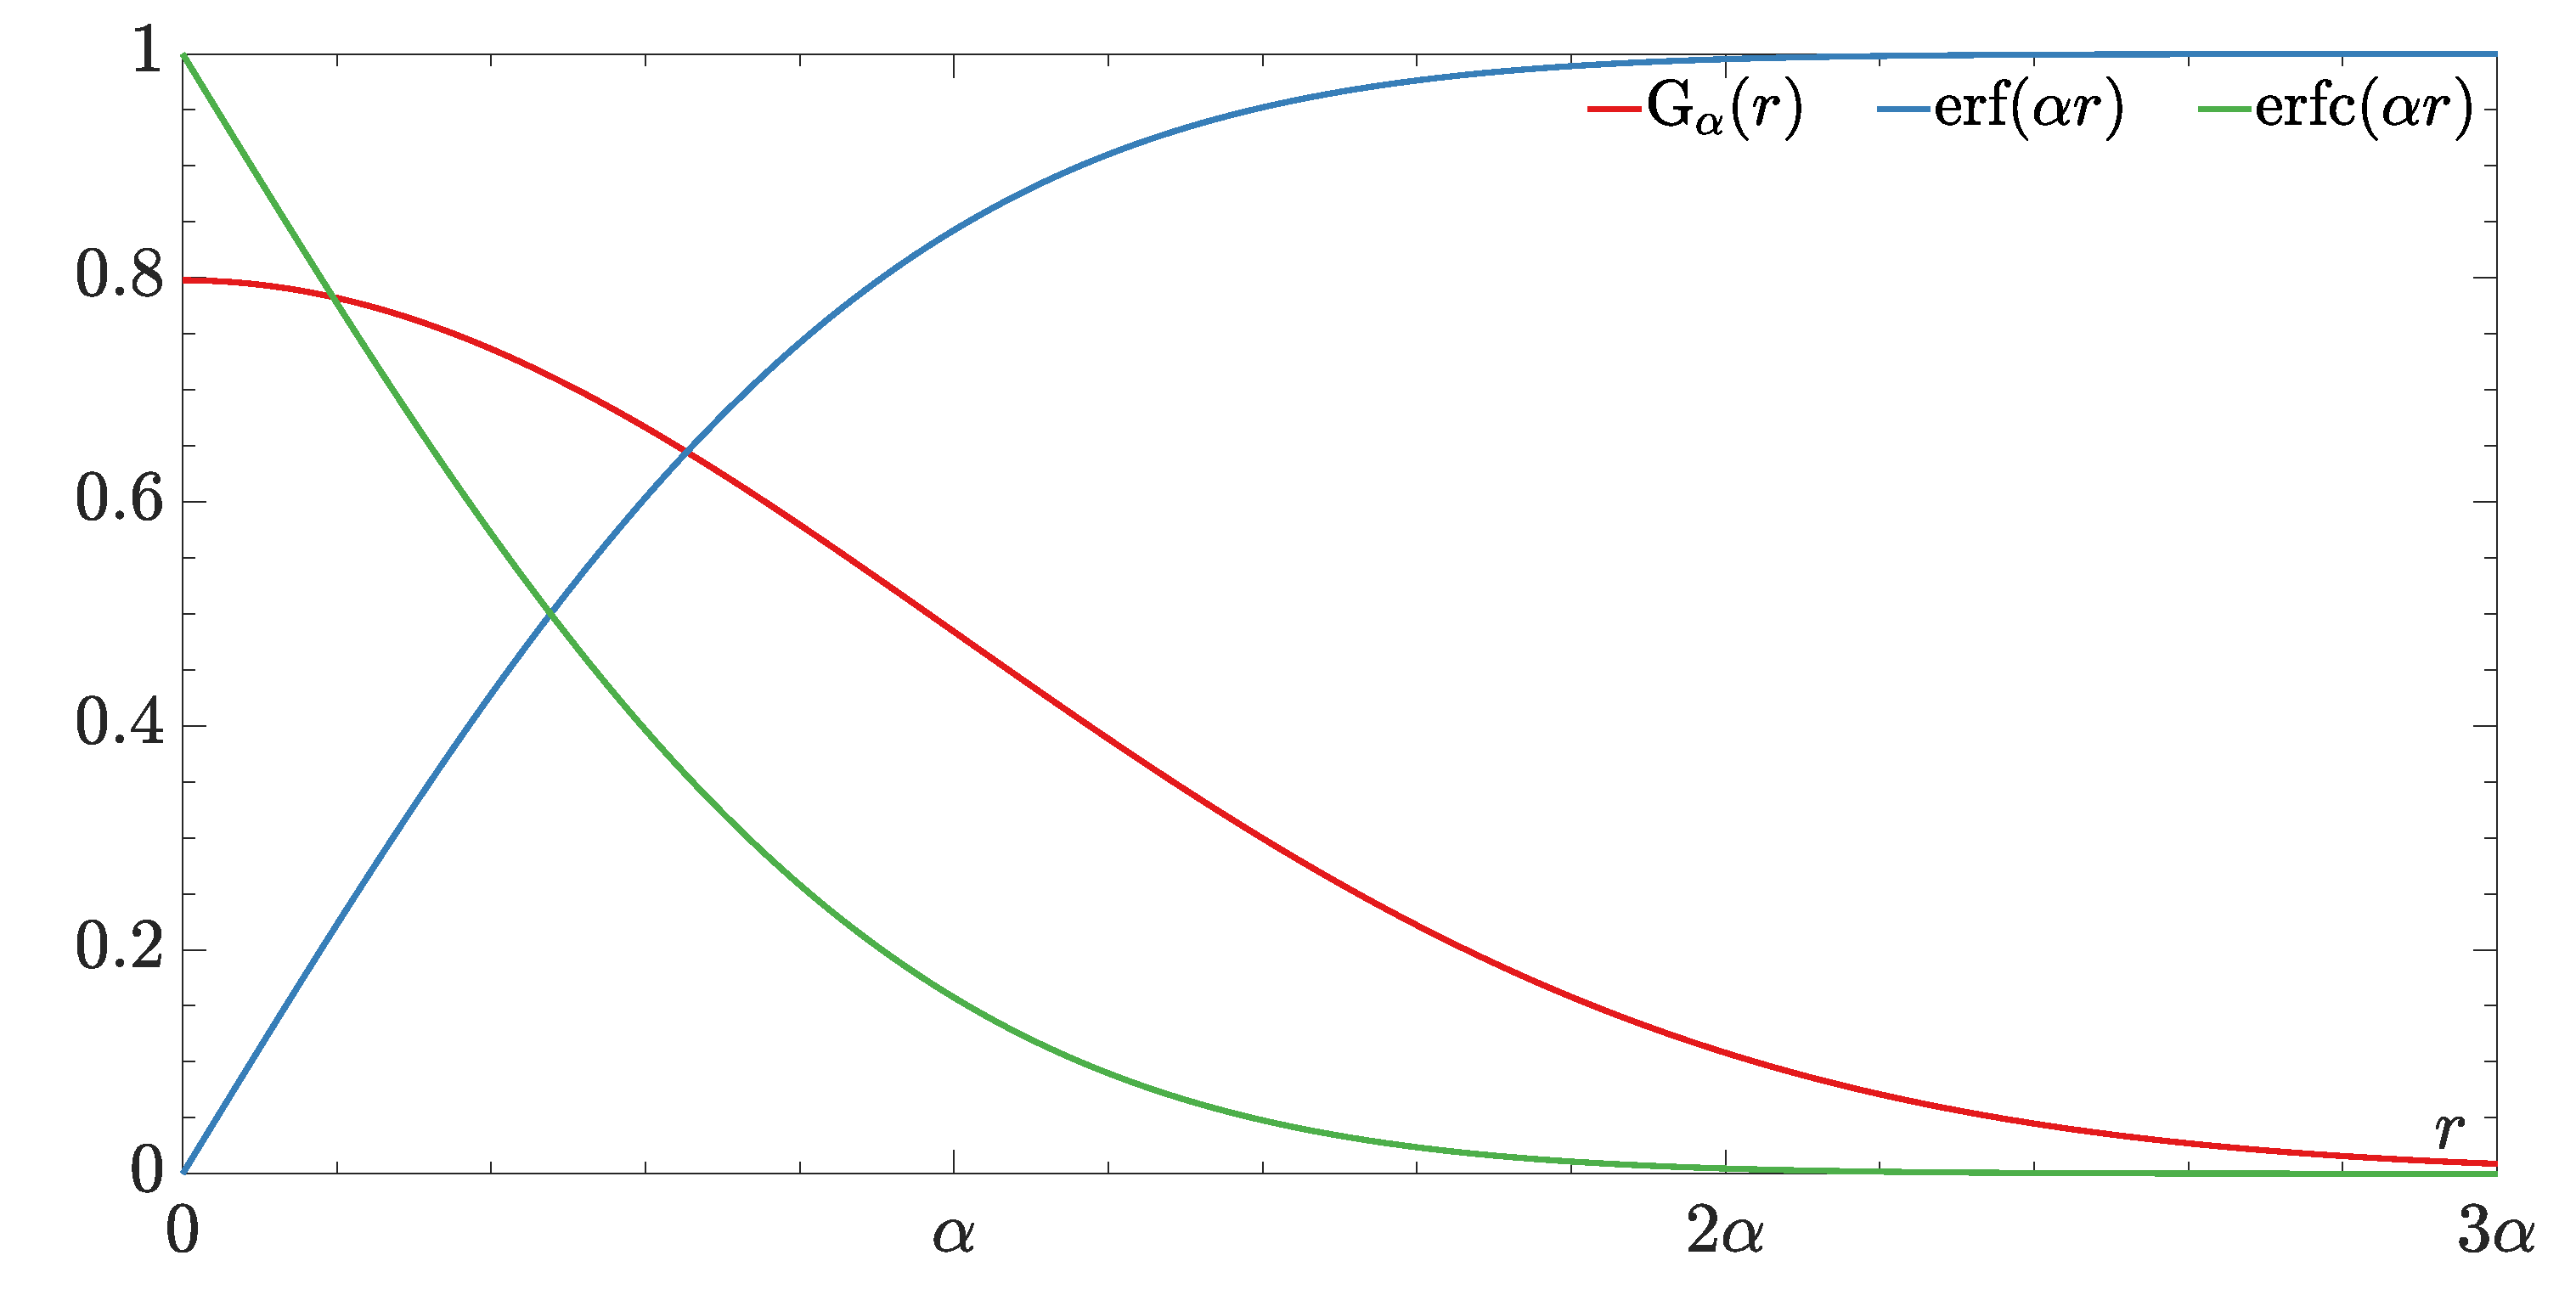
\includegraphics[trim={0cm 0cm 0cm 0cm},clip,width=\textwidth]{figures/Error_Functions.eps}
\end{center}
\end{frame}

\begin{frame}
\frametitle{Ewald Summation}
\begin{center}
	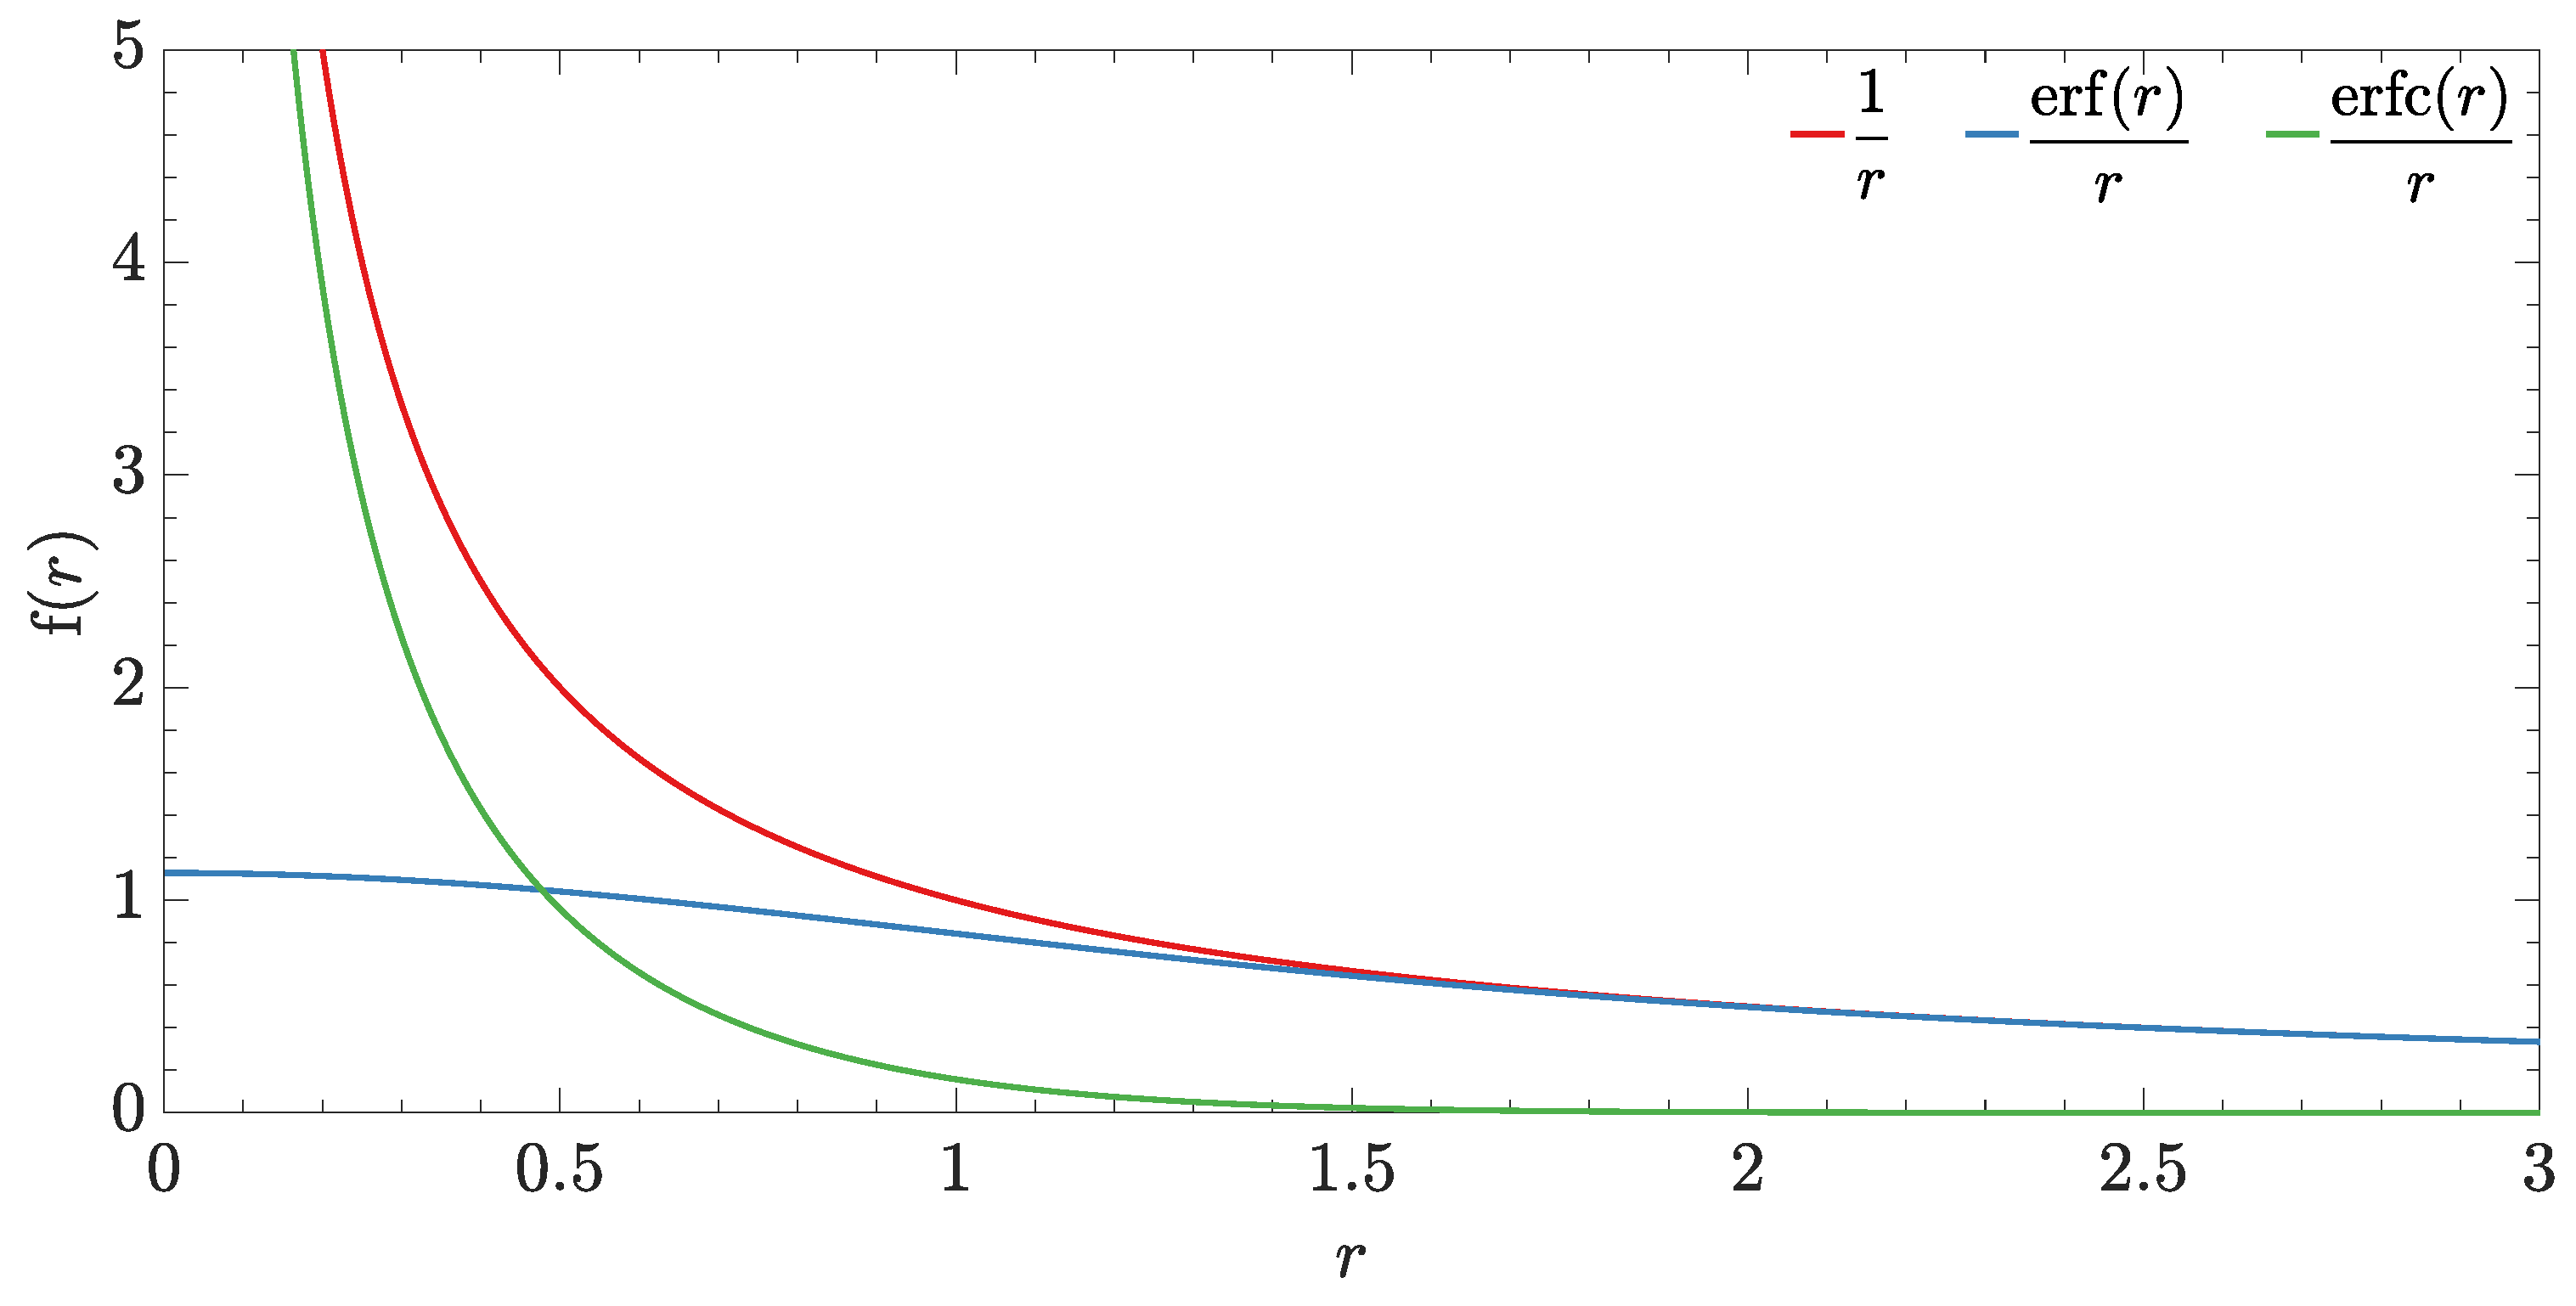
\includegraphics[trim={0cm 0cm 0cm 0cm},clip,width=0.8\textwidth]{figures/Screened_Charges.eps}
\end{center}
The basic idea is to separate the fast variation part for small r and the smooth part for large r. In particular,
the first part should decay fast and be negligible beyond some cutoff distance, whereas the second part
should be smooth for all r, such that its Fourier transform can be represented by a few terms.
\end{frame}

\currentcitation{\cite{born1918absolute}}
\begin{frame}
\frametitle{Born–Land\'{e} Equation from 1918}
An early attempt at constructing an equation for the lattice energy came form the Born–Land\'{e} model, which hypothesized that the crystal energy was
\begin{align*}
E (r) = \frac { M Z ^ { + } Z ^ { - } e ^ { 2 } } { 4 \pi \epsilon _ { 0 } r } + \frac { B } { r^n }.
\end{align*}
Differentiating with respect to r and solving for the unknown $B$ yields
\begin{align*}
E_{Lattice} = \frac { M Z ^ { + } Z ^ { - } e ^ { 2 } } { 4 \pi \epsilon _ { 0 } r _ { 0 } } \left( 1 - \frac { 1 } { n } \right).
\end{align*}
\end{frame}

\currentcitation{\cite{Huggins1937}}
\begin{frame}
\frametitle{Born-Mayer Equation from 1932}
A slightly better attempt at an equation for the lattice energy came form the Born-Mayer model,
\begin{align*}
E (r) = \frac { M Z ^ { + } Z ^ { - } e ^ { 2 } } { 4 \pi \epsilon _ { 0 } r } + B \exp\big(\frac{-r}{\rho}\big).
\end{align*}
Differentiating with respect to r and solving for the unknown $B$ yields
\begin{align*}
E_{Lattice} =  \frac { M Z ^ { + } Z ^ { - } e ^ { 2 } } { 4 \pi \epsilon _ { 0 } r _ { 0 } } \left( 1 - \frac { \rho } { r _ { 0 } } \right).
\end{align*}
\end{frame}

\currentcitation{\cite{Jenkins2005}}
\begin{frame}
\frametitle{Born-Haber Cycle for Lattice Energies}
\begin{columns}
	\begin{column}{0.7\textwidth}
	\begin{center}
		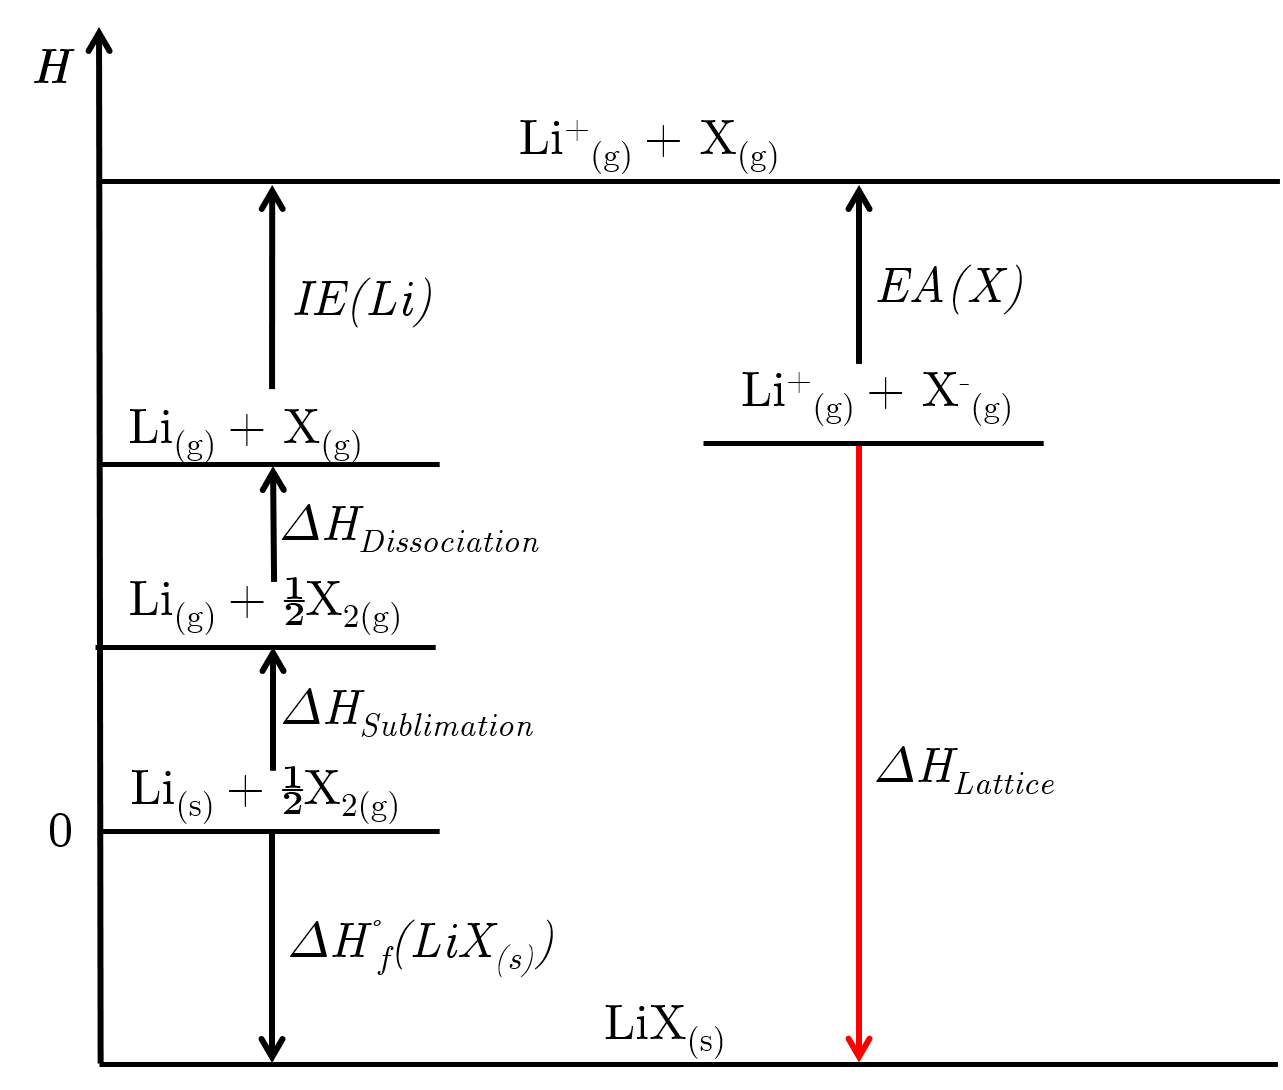
\includegraphics[trim={0cm 0cm 0cm 0cm},clip,width=\textwidth]{figures/Born_Haber.png}
	\end{center}
	\end{column}
	\begin{column}{0.3\textwidth}
		\textbf{Experimental Lattice Enthalpies}
		\begin{align*}
			\Delta &H_{Lattice} =\\ & \Delta H^{\circ}_{f} (LiX_{(s)})\\ &+ \Delta H_{Sub} (Li)\\ &+ \Delta H_{Dissociation} (X_{2})\\ &+ IE (Li)\\ &- EA (X)
		\end{align*}
	\end{column}
\end{columns}
\end{frame}

\begin{frame}
\frametitle{Lattice Enthalpy vs Energy}
\begin{center}
	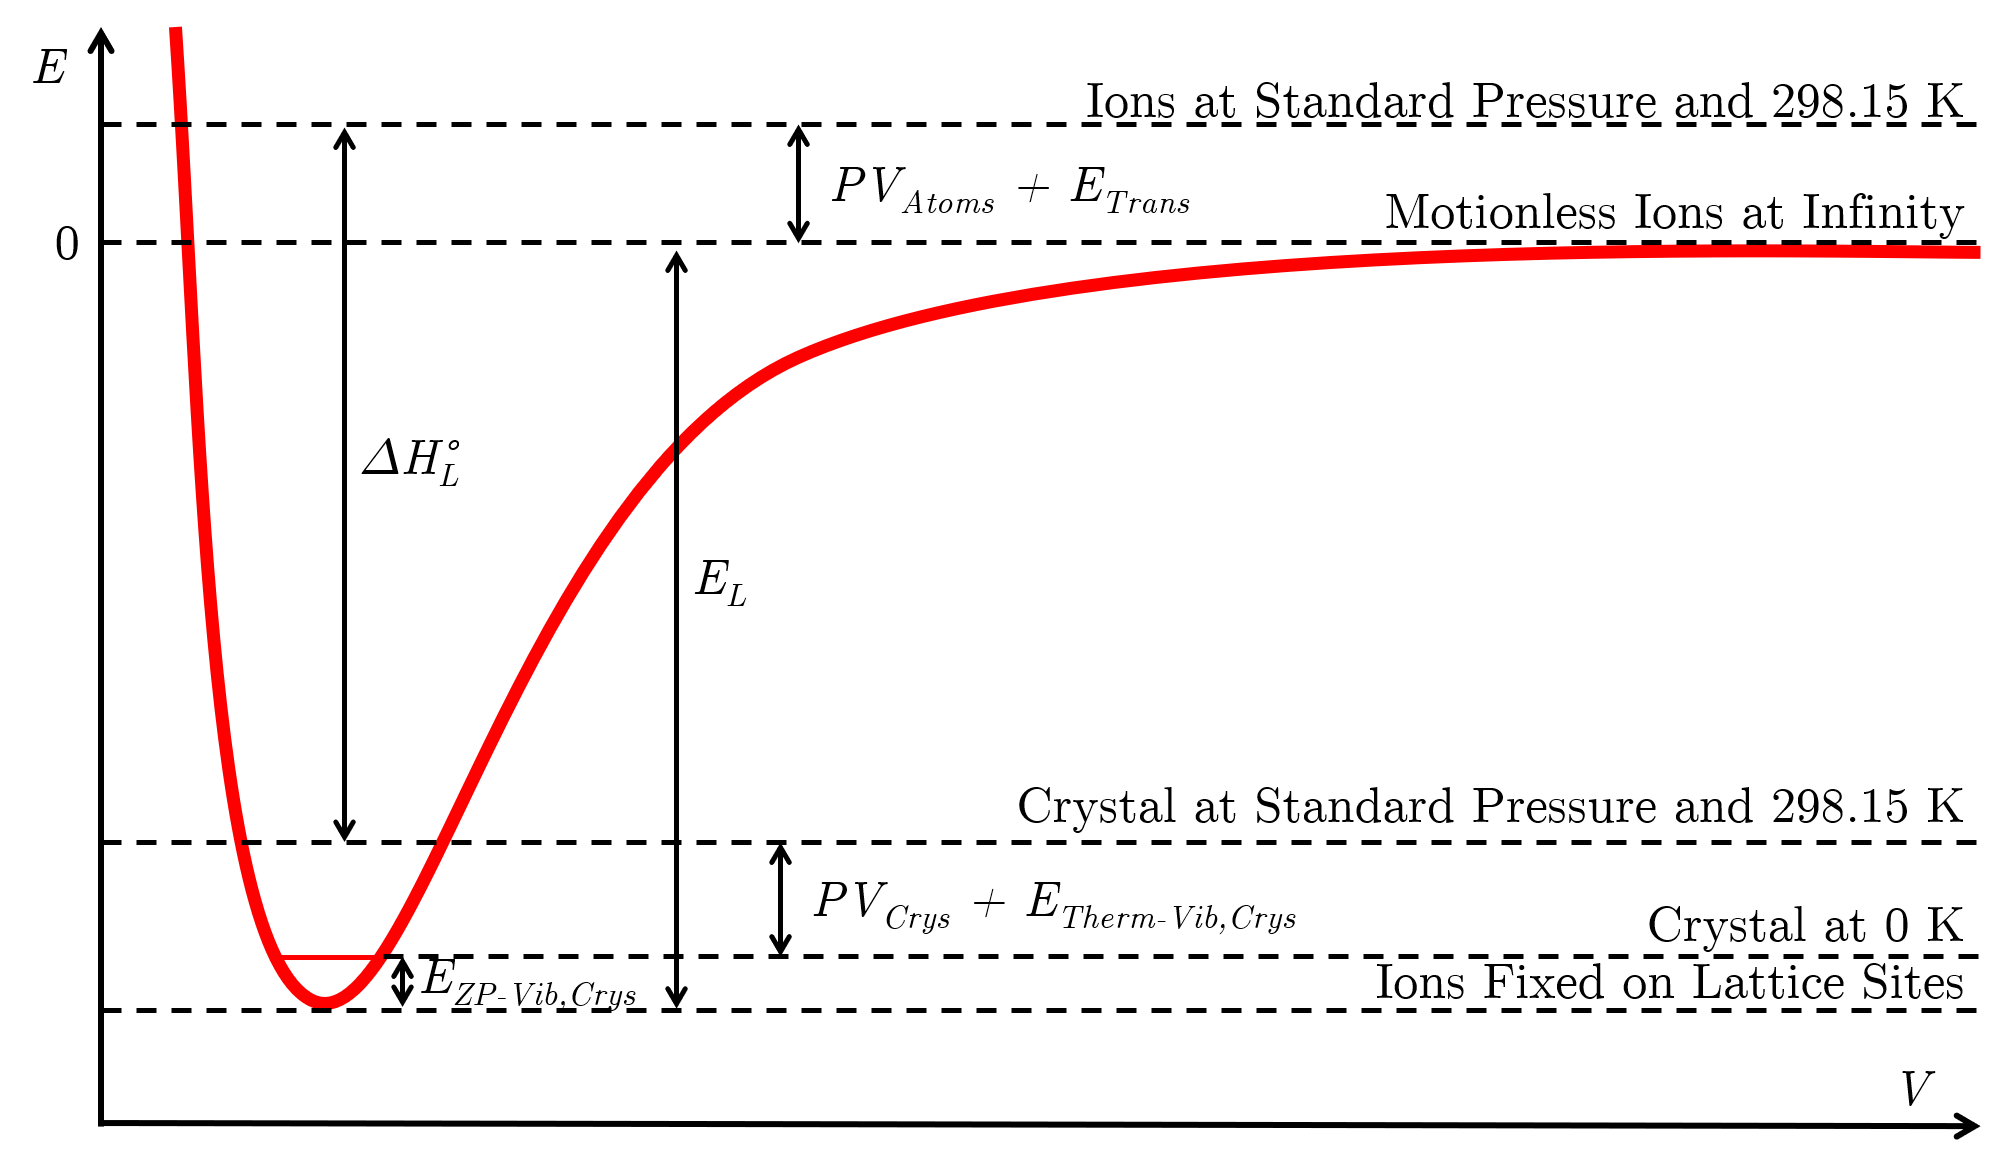
\includegraphics[trim={0cm 0cm 0cm 0cm},clip,width=\textwidth]{figures/Lattice_Energy.png}
\end{center}
\end{frame}

\begin{frame}
\frametitle{Lattice Energy from Enthalpy}
\begin{align*}
\Delta H_{Lattice} &=  H_{Crystal} - H_{Ions} \\
&= E_{Crystal} + (PV)_{Crystal} - E_{Ions} - (PV)_{Ions}.
\end{align*}
Assume $P_{Crystal}$ = $P_{Ions} = P = 1 bar$ and constant $T = 298.15$.
\begin{align*}
\Delta H_{Lattice} &= V_{Crystal} + E_{ZP} + E_{Vib} + PV_{Crystal} - V_{Ions} - E_{Trans} - PV_{Ions}\\
&= E_{Lattice} + E_{ZP} + E_{Vib} - E_{Trans} + P\Delta V .
\end{align*}
Assume the molar volume of the crystal is 0, and assume ions are ideal so $PV = nRT$.
\begin{align*}
\Delta H_{Lattice} &= E_{Lattice} + E_{ZP} + E_{Vib} - E_{Trans} + \Delta n RT 
\end{align*}
where $\Delta n = (- n_{ions})$.
\end{frame}

\begin{frame}
\frametitle{Lattice Energy from Enthalpy}
So ignoring volume of crystal, assuming ideal gas behaviour, and assuming constant $T$ and $P$ we have for a salt M$_{a}$X$_{b}$
\begin{align*}
E_{Lattice} = \Delta H_{Lattice} - E_{ZP} - E_{Vib} + E_{Trans} + (a + b) RT .
\end{align*}
In practice the zero point vib. energy is ignored, and the vibrational energy is assumed $E_{Vib} = 3 n R T$ (high T classical limit). Likewise, the ions translational energy is assumed $E_{Trans} = \frac{3}{2} n R T$ yielding
\begin{align*}
E_{Lattice} &= \Delta H_{Lattice} - 3 (a + b) R T + \frac{3}{2} (a + b) R T + (a + b) R T \\
E_{Lattice} &= \Delta H_{Lattice} - \left[ a \left( \frac { 3 } { 2 } - 2 \right) + b \left( \frac { 3 } { 2 } - 2 \right) \right] R T.
\end{align*}
\end{frame}

% Gaussian Basis sets
\currentcitation{}
\begin{frame}
\frametitle{Gaussian Basis Sets}
In general, molecular orbitals are created by linear combination of atomic orbitals
\begin{equation*}
\Psi _ { i } ( \mathbf { r } ) = \sum _ { \mu = 1 } ^ { K } c _ { \mu i } \Phi_ { \mu } ( \mathbf { r } ) .
\end{equation*}
When using a Gaussian basis set, each atomic orbital is itself a linear combination (a ``contraction'') of 3D primitive Gaussian functions multiplied by a spherical harmonic $Y _ { \ell m } ( \theta , \phi )$, which are centered in space on an atomic nucleus $A$.
\begin{align*}
\Phi_{A} ( \mathbf { r } ) &= R _ { A\ell } ( \mathbf { r } ) Y _ { \ell m } ( \theta , \phi )\\
R _ { A\ell } ( \mathbf { r } ) &= (\mathbf{r} - \mathbf{r_{A}}) ^ { \ell } \sum _ { j } c _ { j } B \left( \ell , \alpha _ { j } \right) \exp \left( - \alpha _ { j } (\mathbf { r } - \mathbf { r_{A} }) ^ { 2 } \right).
\end{align*}
where $B \left( \ell , \alpha _ { j } \right)$ is a normalization constant which insures that $\int d\mathbf { r } \left| B \left( \ell , \alpha _ { j } \right) \exp \left( - \alpha _ { j } (\mathbf { r } - \mathbf { r_{A} }) ^ { 2 } \right) \right| ^ { 2 } = 1$.
\end{frame}

\begin{frame}
\frametitle{Gaussian Basis Sets: Minimal}
\begin{itemize}
\item A minimal basis set is constructed using only one atomic orbital function of each type occupied in the atom(s) of the basis set. 
\item For example, Lithium has $1s^{2}2s{1}$ so a minimal basis set uses two contracted sets of $s$-type Gaussians, one for the $1s$ electrons and one for the $2s$ electron.
\item The most common minimal basis set is STO-$n$G, where $n$ is an integer. 
\item These ``Slater-Type Orbitals'' are each made from a linear combination (contraction) of $n$ primitive Gaussians. Only the minimum number of atomic orbitals are used.
\item Slater orbitals are similar to primitive Gaussians, but have a more physical shape with a \bb{cusp}.
\begin{align*}
R _ { A n} ( \mathbf { r } ) &= (\mathbf { r } - \mathbf { r_{A} }) ^ { n - 1 } N \exp \left( - \xi (\mathbf { r } - \mathbf { r_{A} }) \right).
\end{align*}
\end{itemize}
\end{frame}

\begin{frame}
\frametitle{Gaussian Basis Sets: Slater Orbitals}
\begin{center}
	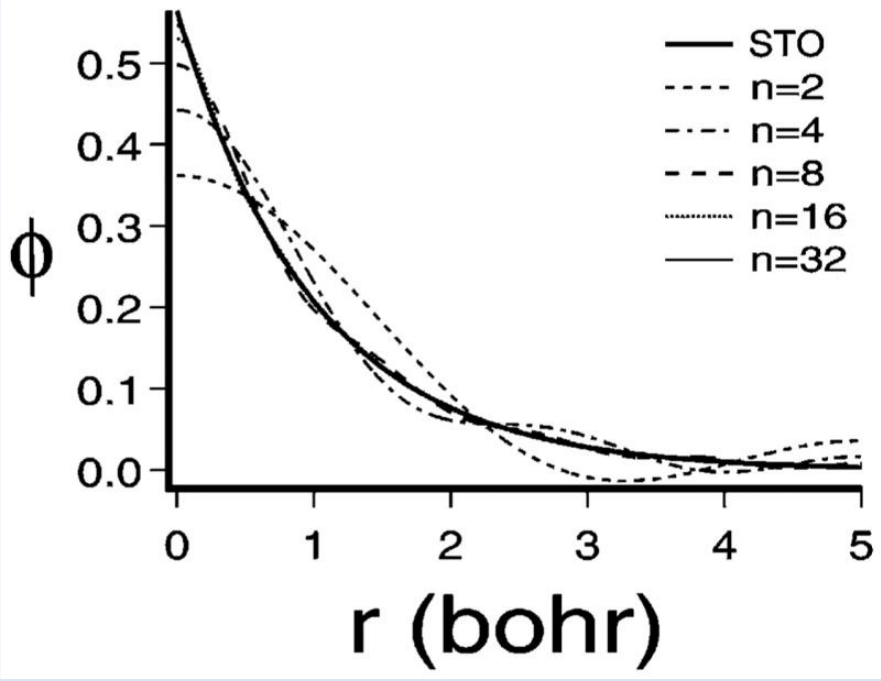
\includegraphics[trim={0cm 0cm 0cm 0cm},clip,width=0.8\textwidth]{figures/Slater_vs_Gaussian.PNG}
\end{center}
\end{frame}

\begin{frame}
\frametitle{Gaussian Basis Sets: Notation}
\begin{itemize}
	\item Core electrons are tightly bound, and are not affected much by nearby atoms.
	\item Split valence: only one basis function for core AOs, and more basis functions for valence AOs
	\item pob-TZVP basis set has so-called ``triple-zeta valence'' quality. This means it has three times as many atomic orbitals as a minimal basis set would for the same atom for the valence orbitals. The core electrons are treated minimally.
	\item The ``P'' in pob-TZVP indicates that there is an additional set of polarization functions. To polarize a basis function with angular momentum $\ell$, one mixes it with basis functions of angular momentum $\ell$ + 1.
	\item Li: one atomic orbital for the $1s$ orbital, three atomic orbitals to describe the valence $2s$ orbital, plus one set of $p$-type Gaussian orbitals for polarization.
\end{itemize}
\end{frame}


\begin{frame}
\frametitle{Gaussian Basis Sets: Pople Notation}
\begin{itemize}
	\item Pople notation is commonly used to describe Gaussian basis sets: usually looks like \bb{$X$-$Y$G}.
	\item \bb{$X$} is an integer that indicates the number of contracted Gaussians used to describe each of the core electrons. Core orbitals are usually described by only one contracted Gaussian each.
	\item \bb{$Y$} is a set of integers such as $311$. The number of integers corresponds to the number of contracted Gaussians used to described the valence orbitals. Each integer in this number is the number of contracted Gaussians in the atomic orbital.
	\item Example: 7-311G has 7 primitive Gaussians contracted into a single function for each core atomic orbital. The valence orbitals each have three functions, the first of which is made of three primitive Gaussians whereas each of the others is made from one primitive Gaussian.
\end{itemize}
\end{frame}

\begin{frame}
\frametitle{Gaussian Basis Sets: Extra Notation}
\begin{itemize}
	\item Correlation consistent basis sets are augmented with successively larger shells of polarization. They are required for good quality post-HF calculations.
	\item `cc-p', stands for `correlation consistent polarized'.
	\item The prefix `aug' means that the basis is augmented with diffuse functions, which more	accurately represent the ``tail'' portion of the atomic orbitals.
	\item In pople notation * means extra polarization functions on non-H atoms, while ** includes H atoms.
	\item Similarly, + and ++ correspond to extra diffuse functions.
\end{itemize}
\end{frame}


% XC FUNCTIONALS
\currentcitation{}
\begin{frame}
\frametitle{Exchange-Correlation Functionals: Local Density Approximation}
Local spin density approximation (LSDA) XC functionals have the following general form
\begin{equation*}
E _ {LDSA}[\rho_{\downarrow}(\mathbf{r}), \rho_{\uparrow}(\mathbf{r})] = \int \rho(\mathbf{r}) \varepsilon^{LDSA}_{XC}[\rho_{\downarrow} (\mathbf{r}), \rho_{\uparrow} (\mathbf{r})]d\mathbf{r}.
\end{equation*}
XC energy density at each point in space assumed same as a homogeneous electron gas (HEG) with that electron density.
\begin{equation*}
 \varepsilon^{LDSA}_{XC}[\rho_{\downarrow} (\mathbf{r}), \rho_{\uparrow} (\mathbf{r})] = \frac{1}{2} \int \rho(\mathbf{r'})\big( \bar{g}^{HEG}[|\mathbf{r} - \mathbf{r'} |,\rho_{\downarrow} (\mathbf{r}), \rho_{\uparrow} (\mathbf{r})] -1 \big)d\mathbf{r'}
\end{equation*}
where $\bar{g}^{HEG}$ is the averaged pair-correlation function in the homogeneous electron gas. $\rho (\mathbf{r}) = \rho_{\downarrow} (\mathbf{r}) + \rho_{\uparrow}(\mathbf{r})$.
\end{frame}


\currentcitation{}
\begin{frame}
\frametitle{Exchange-Correlation Functionals: Generalized Gradient Approximation}
Improves on LSDA in the spirit of a Taylor expansion: depends on $\rho (r)$ but also $\nabla \rho (r)$
\begin{equation*}
E _ { GGA } \left[ \rho _ { \uparrow }(\mathbf{r}) , \rho _ { \downarrow }(\mathbf{r}) \right] = \int  f \left( \rho _ { \uparrow }(\mathbf{r}) , \rho _ { \downarrow }(\mathbf{r}) , \nabla \rho _ { \uparrow }(\mathbf{r}) , \nabla \rho _ { \downarrow }(\mathbf{r}) \right) d \mathbf{r}
\end{equation*}
where the function $f$ depends on the particular GGA XC functional. $f$ is usually designed such that
\begin{equation*}
f \left( \rho _ { \uparrow }(\mathbf{r}) , \rho _ { \downarrow }(\mathbf{r}) , 0 , 0 \right) = \rho (\mathbf{r}) \varepsilon^{LDSA}_{XC}[\rho_{\downarrow} (\mathbf{r}), \rho_{\uparrow} (\mathbf{r})]
\end{equation*}
\end{frame}


\currentcitation{\cite{Perdew1996}}
\begin{frame}
\frametitle{Exchange-Correlation Functionals: PBE}
\begin{itemize}
	\item Generalized Gradient Approximation class of XC functional.
	\item Designed to be entirely free of empirical parameters, while satisfying many energetically-significant conditions.
\end{itemize}
\end{frame}


% AB INITIO DETAILS
\currentcitation{}
\begin{frame}
\frametitle{Method: Ab Initio Calculations}
Comparison of Ab Initio methods:
\begin{columns}
	\begin{column}{0.33\textwidth}
		\bb{HF Theory:}
		\begin{itemize}
			\item Exact Coulomb.
			\item Exact Exchange.
			\item No Correlation.
			\item Mean-field.
			\item Scales $N^{4}$.
		\end{itemize}
	\end{column}
	\begin{column}{0.36\textwidth}
		\rule{0pt}{4.5ex}    
		\bb{DFT:}
		\begin{itemize}
			\item Exact Coulomb.
			\item Approx. Exchange.
			\item Approx. Correlation.
			\item Scales $N^{3}$ or $N^{4}$.
			\item Based on electron density.
		\end{itemize}
	\end{column}
	\begin{column}{0.33\textwidth}
		\rule{0pt}{4.5ex}
		\bb{Post-HF Methods:}
		\begin{itemize}
			\item Exact Coulomb.
			\item Exact Exchange.
			\item Accurate Approx. Correlation.
			\item Poor Scaling, often huge calculations.
		\end{itemize}
	\end{column}
\end{columns}
\begin{itemize}
	\item Born-Oppenheimer approximation, neglect relativistic effects, incomplete basis Sets, and numerical approximations.
\end{itemize}
\end{frame}

\begin{frame}
\frametitle{BSSE}
\begin{center}
\includegraphics[trim={0cm 0cm 0cm 0cm},clip,width=\textwidth]{\figfile/BSSE_PBE.eps}
\end{center}
\end{frame}

\begin{frame}
\frametitle{Zero T Pressure vs a}
\begin{center}
	\includegraphics[trim={0cm 0cm 0cm 0cm},clip,width=\textwidth]{\figfile/a_vs_P.eps}
\end{center}
\end{frame}

\currentcitation{Lanaro, G. and G. N. Patey, J. Chem. Phys. \textbf{146}, 154501 (2017)}
\begin{frame}
\frametitle{Comparison of LiX Rocksalt vs Wurtzite for TF and JC}
\begin{center}
	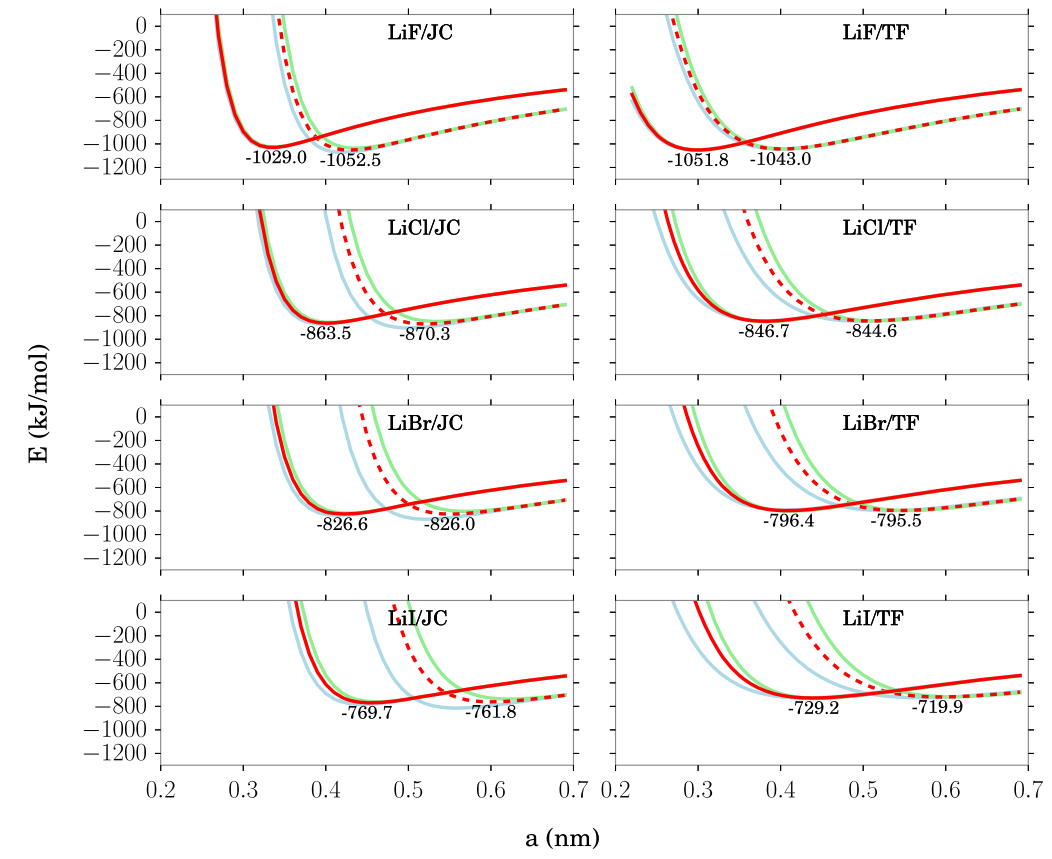
\includegraphics[trim={0cm 0cm 0cm 0cm},clip,width=0.8\textwidth]{figures/JC_vs_TF.png}
\end{center}
\end{frame}

% DISPERSION
\currentcitation{E. Johnson and A. Becke, J. Chem. Phys. \textbf{124}, 174104 (2006)}
\begin{frame}
\frametitle{Importance of Dispersion}
DFT does not take into account dispersion at large r: asymptotic interaction energy of local density functionals falls off exponentially.
\begin{alertblock}{One solution:}
	Third generation dispersion (D3) with Becke-Johnson damping function:
\end{alertblock}
\begin{equation*}
E _ { \text { disp } } = - \sum _ { i > j } \bigg( \frac { C _ { 6 , i j } } { R _ { \text {vdW}, i j } ^ { 6 } + R _ { i j } ^ { 6 } } + \frac { C _ { 8 , i j } } { R _ { \text {vdW}, i j } ^ { 8 } + R _ { i j } ^ { 8 } } + \frac { C _ { 10 , i j } } { R _ { \text {vdW}, i j } ^ { 10 } + R _ { i j } ^ { 10 } } \bigg) 
\end{equation*}
\begin{itemize}
	\item $C_{n,ij}$ are parameter free, calculated on the fly from occupied orbitals and polarizabilities. Therefore, $C_{n,ij}$ change with the electronic environment.
	\item $R _ { \text {vdW}, i j }$ = sum of effective VdW radii of atoms $i$ and $j$.
\end{itemize}
\end{frame}

% CRYSTAL STRUCTURES
\currentcitation{}
\begin{frame}
\frametitle{Rocksalt}
\begin{columns}
	\begin{column}{0.5\textwidth}
		\begin{center}
			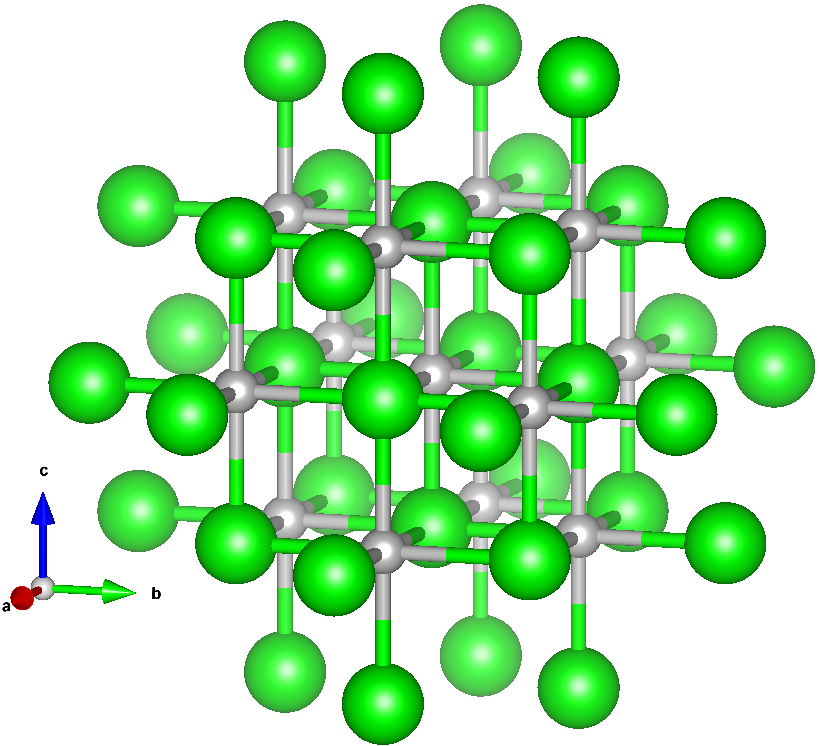
\includegraphics[trim={0cm 0cm 0cm 0cm},clip,width=\textwidth]{figures/Rocksalt.png}
		\end{center}
	\end{column}
	\begin{column}{0.5\textwidth}
	\begin{itemize}
		\item Face centered cubic
		\item Space Group: Fm$\bar{3}$m (225)
		\item $a = b = c$
		\item $\alpha = \beta = \gamma = 90^{\circ}$
		\item 8 Atoms in Unit Cell
		\item 2 Atoms in Asym. Unit
		\item Coordination number: 6
		\item Nearest Neighbour bond length: $\frac{1}{2}a$
		\item Fractional Coordinates: \mbox{Li = $(0, 0, 0)$} and \mbox{X = $(\frac{1}{2}, 0, 0)$}
	\end{itemize}
	\end{column}
\end{columns}
\end{frame}

\begin{frame}
\frametitle{Wurtzite}
\begin{columns}
	\begin{column}{0.5\textwidth}
		\begin{center}
			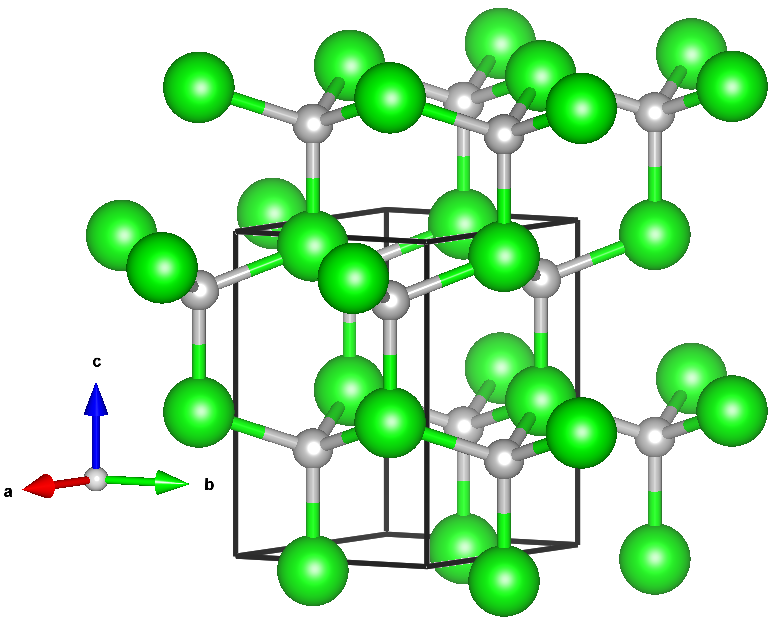
\includegraphics[trim={0cm 0cm 0cm 0cm},clip,width=\textwidth]{figures/Wurtzite.png}
		\end{center}
	\end{column}
	\begin{column}{0.5\textwidth}
		\begin{itemize}
			\item Primitive Hexagonal
			\item Space Group: P$6_{3}$mc (186)
			\item $a = b = \sqrt{\frac{3}{8}}c$
			\item $\alpha = \beta = 90^{\circ}$; $\gamma = 120^{\circ}$
			\item 4 Atoms in Unit Cell
			\item 2 Atoms in Asym. Unit
			\item Coordination number: 4
			\item Nearest Neighbour bond length: $\sqrt{\frac{3}{8}}a$
			\item Fractional Coordinates: \mbox{Li = $(\frac{1}{3}, \frac{2}{3}, \frac{3}{8})$} and \mbox{X = $(\frac{1}{3}, \frac{2}{3}, 0)$}
		\end{itemize}
	\end{column}
\end{columns}
\end{frame}

\begin{frame}
\frametitle{Sphalerite (Zincblende)}
\begin{columns}
	\begin{column}{0.5\textwidth}
		\begin{center}
			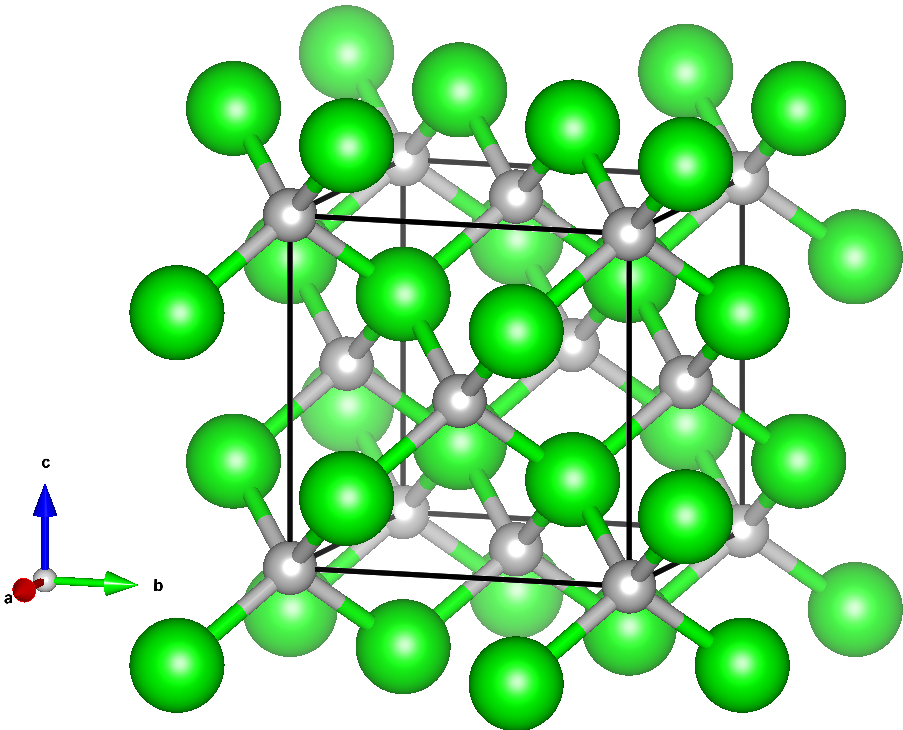
\includegraphics[trim={0cm 0cm 0cm 0cm},clip,width=\textwidth]{figures/Sphalerite.png}
		\end{center}
	\end{column}
	\begin{column}{0.5\textwidth}
		\begin{itemize}
			\item Face Centered Cubic
			\item Space Group: F$\bar{4}$3m (216)
			\item $a = b = c$
			\item $\alpha = \beta = \gamma = 90^{\circ}$
			\item 8 Atoms in Unit Cell
			\item 2 Atoms in Asym. Unit
			\item Coordination number: 4
			\item Nearest Neighbour bond length: $\frac{\sqrt{3}}{4}a$
			\item Fractional Coordinates: \mbox{Li = $(0, 0, 0)$} and \mbox{X = $(\frac{1}{4}, \frac{1}{4}, \frac{1}{4})$}
		\end{itemize}
	\end{column}
\end{columns}
\end{frame}

\begin{frame}
\frametitle{NiAs (B8$_1$)}
\begin{columns}
	\begin{column}{0.5\textwidth}
		\begin{center}
			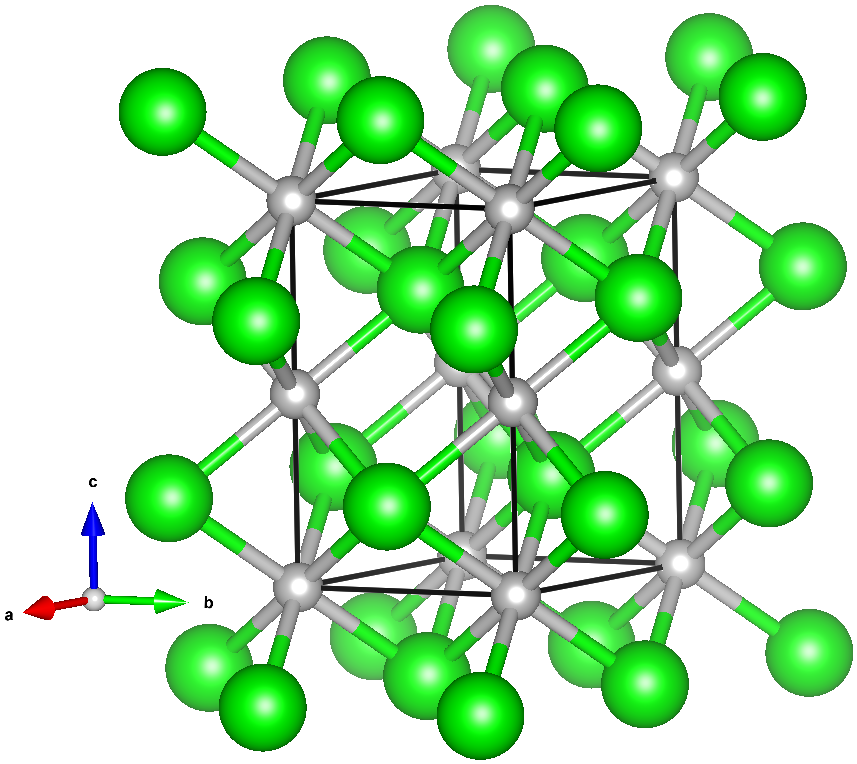
\includegraphics[trim={0cm 0cm 0cm 0cm},clip,width=\textwidth]{figures/NiAs.png}
		\end{center}
	\end{column}
	\begin{column}{0.5\textwidth}
		\begin{itemize}
			\item Primitive Hexagonal
			\item Space Group: P$\frac{6_{3}}{m}$mc (194)
			\item $a = b; c \approx 1.39 a$ (variable)
			\item $\alpha = \beta = 90^{\circ}; \gamma = 120^{\circ}$
			\item 4 Atoms in Unit Cell
			\item 2 Atoms in Asym. Unit
			\item Coordination number: 6
			\item Nearest Neighbour bond length: $\sqrt{\frac{a^2}{3} + \frac{c^2}{16}}$
			\item Fractional Coordinates: \mbox{Li = $(0, 0, 0)$} and \mbox{X = $(\frac{1}{3}, \frac{2}{3}, \frac{1}{4})$}
		\end{itemize}
	\end{column}
\end{columns}
\end{frame}

\begin{frame}
\frametitle{5-5}
\begin{columns}
	\begin{column}{0.5\textwidth}
		\begin{center}
			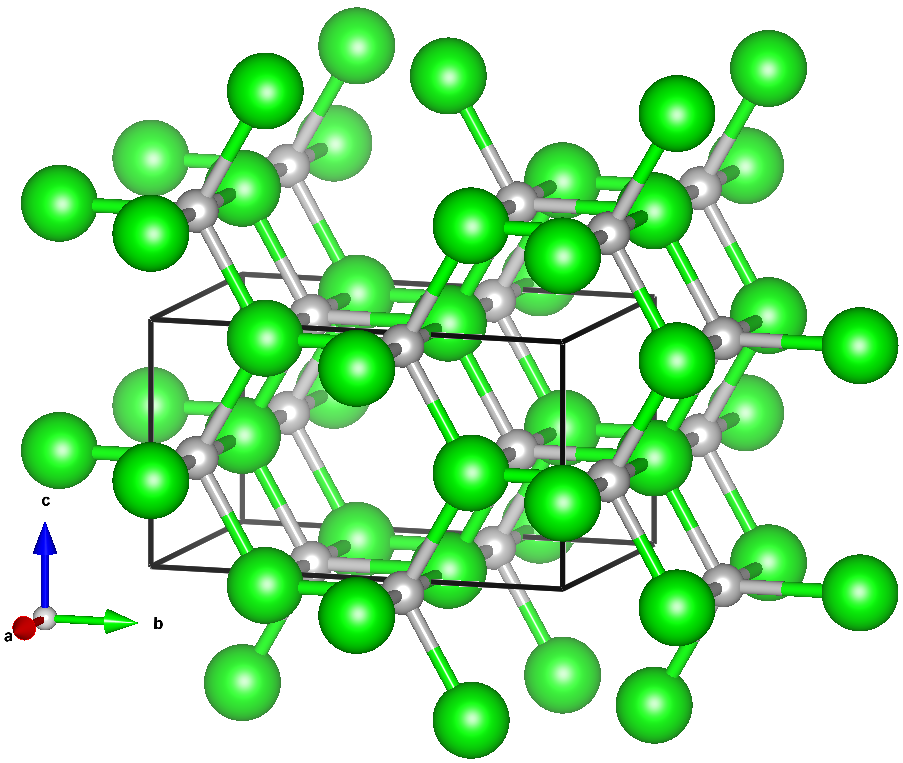
\includegraphics[trim={0cm 0cm 0cm 0cm},clip,width=\textwidth]{figures/5-5.png}
		\end{center}
	\end{column}
	\begin{column}{0.5\textwidth}
		\begin{itemize}
			\item Primitive Orthorhombic
			\item Space Group: Pnnm (58)
			\item $a = \frac{2}{3}b = \frac{2}{\sqrt{3}}c$
			\item $\alpha = \beta = \gamma = 90^{\circ}$
			\item 8 Atoms in Unit Cell
			\item 2 Atoms in Asym. Unit
			\item Coordination number: 5
			\item Nearest Neighbour bond length: $\frac{1}{2}a$
			\item Fractional Coordinates: \mbox{Li = $(\frac{1}{4}, \frac{1}{6}, \frac{1}{2})$} and \mbox{X = $(\frac{1}{4}, \frac{1}{3}, 0)$}
		\end{itemize}
	\end{column}
\end{columns}
\end{frame}

\begin{frame}
\frametitle{CsCl}
\begin{columns}
	\begin{column}{0.5\textwidth}
		\begin{center}
			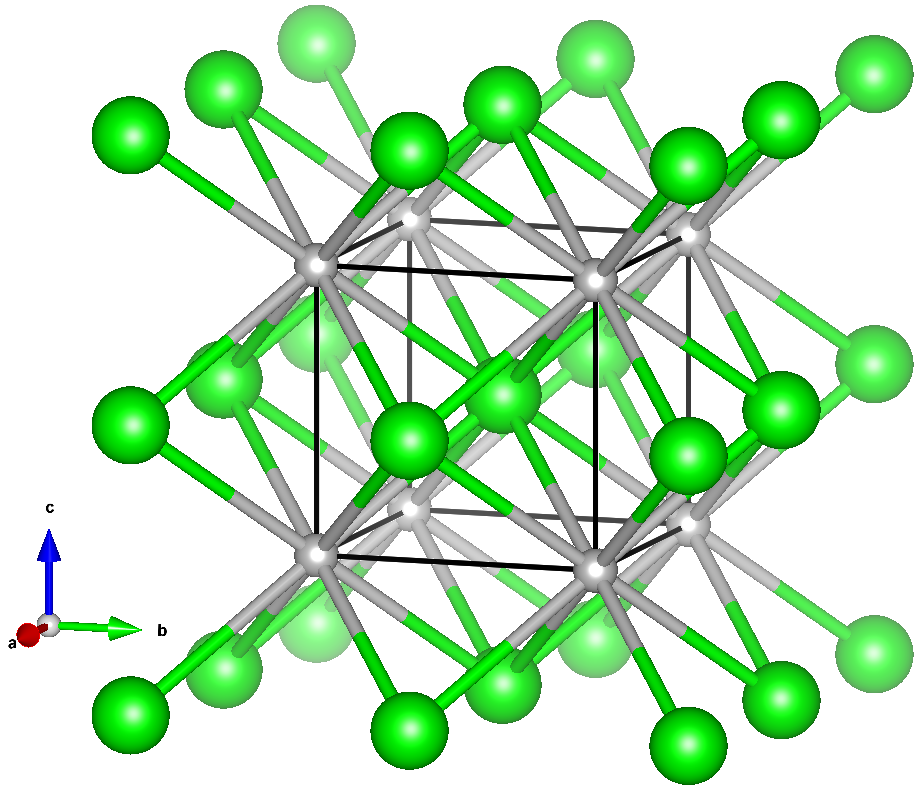
\includegraphics[trim={0cm 0cm 0cm 0cm},clip,width=\textwidth]{figures/CsCl.png}
		\end{center}
	\end{column}
	\begin{column}{0.5\textwidth}
		\begin{itemize}
			\item Primitive Cubic
			\item Space Group: Pm$\bar{3}$m (221)
			\item $a = b = c$
			\item $\alpha = \beta = \gamma = 90^{\circ}$
			\item 2 Atoms in Unit Cell
			\item 2 Atoms in Asym. Unit
			\item Coordination number: 8
			\item Nearest Neighbour bond length: $\frac{\sqrt{3}}{2}a$
			\item Fractional Coordinates: \mbox{Li = $(0, 0, 0)$} and \mbox{X = $(\frac{1}{2}, \frac{1}{2}, \frac{1}{2})$}
		\end{itemize}
	\end{column}
\end{columns}
\end{frame}


% LiF Solubility
\currentcitation{\cite{Booth1950}}
\begin{frame}
\begin{center}
	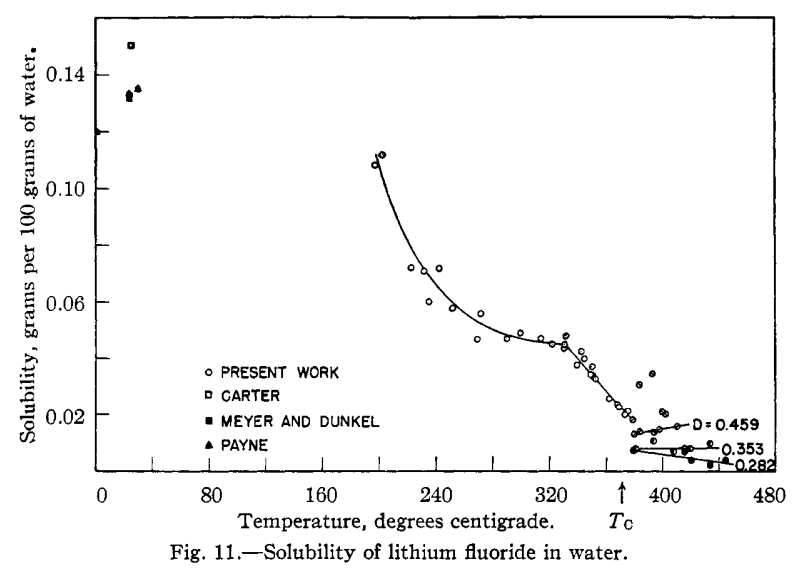
\includegraphics[trim={0cm 0cm 0cm 0cm},clip,width=\textwidth]{figures/LiF_Solubility.PNG}
\end{center}
\end{frame}

% Radius Ratio Rules
\currentcitation{}
\begin{frame}
\frametitle{Radius Ratio Rules}
From traditional ionic radii:
\begin{table}[]
	\begin{tabular}{lll}
		Salt & Radius Ratio & Predicted Structure \\
		LiF & 0.7563 & Primitive Cubic (CsCl) \\
		LiCl & 0.5389 & Rocksalt \\
		LiBr & 0.4945 & Rocksalt \\
		LiI & 0.4369 & Rocksalt \\
		NaCl & 0.6949 & Rocksalt
	\end{tabular}
\end{table}
\end{frame}

\begin{frame}
\frametitle{Radius Ratio Rules}
Using JC $\sigma$ parameter as the ``radius'':
\begin{table}[]
	\begin{tabular}{llll}
		Salt & Radius Ratio & Predicted Structure & Observed Structure\\
		LiF & 0.3505 & Wurtzite &  Rocksalt\\
		LiCl & 0.2918 & Wurtzite & Rocksalt \\
		LiBr & 0.2875 & Wurtzite & Wurtzite \\
		LiI & 0.2710 & Wurtzite & Wurtzite \\
		NaCl & 0.4471 & Rocksalt & Rocksalt
	\end{tabular}
\end{table}
\end{frame}

% NaCl Nucleation crystallinity
\currentcitation{\cite{Lanaro2016}}
\begin{frame}
\frametitle{NaCl Nucleation vs Size and Crystallinity}
\begin{center}
	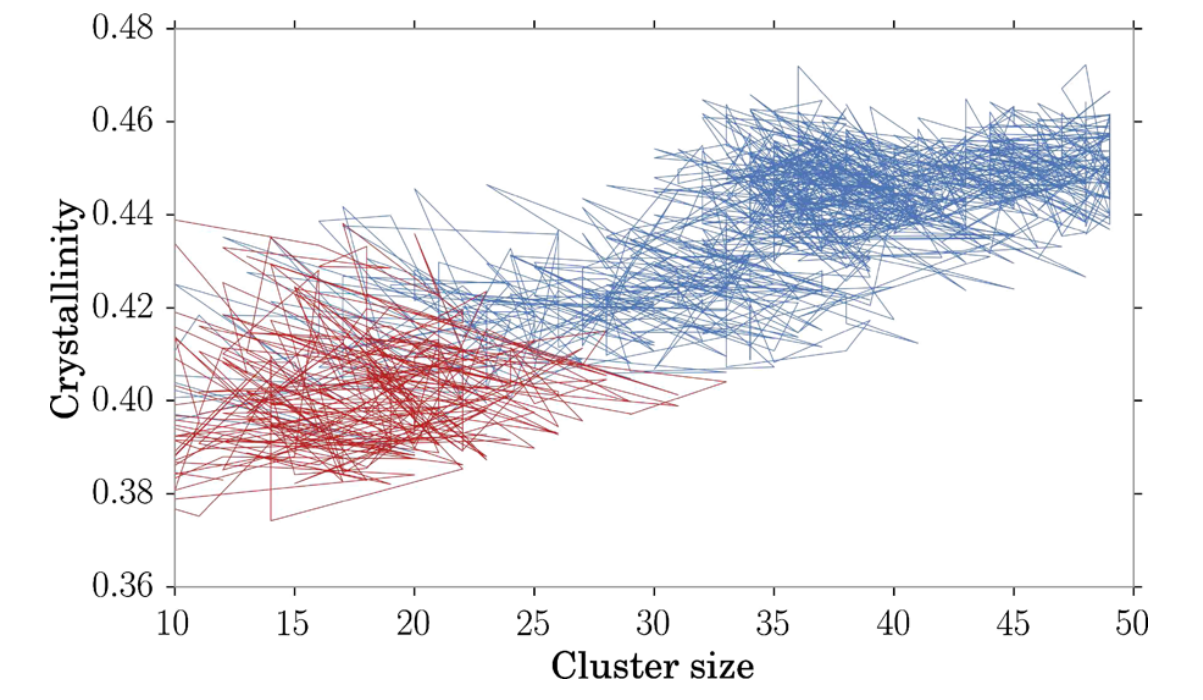
\includegraphics[trim={0cm 0cm 0cm 0cm},clip,width=0.9\textwidth]{figures/Crystallinity.png}
\end{center}
Failed nucleation clusters are shown in red, while successful nucleation clusters are shown in blue.
\end{frame}

\begin{frame}
\frametitle{NaCl Nucleation vs Size and Crystallinity}
The dependence on size is in agreement with CNT, but crystallinity is defined as the average of $q_{8}$ over an entire cluster. For a particular ion,
\begin{align*}
q _ { l } = \left[ \frac { 4 \pi } { 2 l + 1 } \sum _ { m = - l } ^ { l } \left| q _ { l m } \right| ^ { 2 } \right] ^ { 1 / 2 }
\end{align*}
and
\begin{align*}
q _ { l _ { m } } = \frac { 1 } { N } \sum _ { r _ { i } = r _ { 1 } } ^ { r _ { N } } Y _ { l } ^ { m } \left( \theta \left( \mathbf { r } _ { i } \right) , \phi \left( \mathbf { r } _ { i } \right) \right).
\end{align*}
The number 8 was chosen empirically for best separation between liquid and solid phase ions. Here $N=12$ is the number of nearest neighbor ions.
\end{frame}

% Combining rules
\currentcitation{}
\begin{frame}
\frametitle{Lorenz-Berthelot combining rules}
In the JC model, Lennard-Jones parameters are only defined between ions/atoms of the same type. To find the parameters for mixed interactions, the Lorenz-Berthelot combining rules are used:
\begin{align*}
\sigma_{ij} &= \frac{\sigma_{i} + \sigma_{j}}{2}\\
\epsilon_{ij} &= \sqrt{\epsilon_{i} \epsilon_{j}}
\end{align*}
So the radius of the Lennard-Jones well is the arithmetic mean of the two radii, and the well depth is the geometric mean.
\end{frame}

% Basic Thermodynamics
\currentcitation{}
\begin{frame}
\frametitle{The Gibbs Relations}
The first law of thermodynamics states $dU = \dbar q + \dbar w$. For a reversible process, $\dbar q = \frac{dS}{T}$ and $\dbar w = -P dV$, hence
\begin{align*}
	dU = TdS - PdV
\end{align*}
for tiny changes in the internal energy ``at equilibrium.''
From this, increments of $H \equiv U + PV$; $A \equiv U - TS$; and $G \equiv H - TS$ can be similarly defined:
\begin{align*}
dH &= TdS + VdP,\\
dA &= - SdT - PdV,\\
dG &= -SdT + VdP.
\end{align*}
\end{frame}

\begin{frame}
\frametitle{The Gibbs Relations}
From the form of the thermodynamic potentials in differential form:
\begin{align*}
dU &= TdS - PdV,\quad &&dH = TdS + VdP\\
dA &= - SdT - PdV,\quad &&dG = -SdT + VdP.
\end{align*}
We can derive the following mathematical equivalencies
\begin{align*}
&\bigg( \frac{\partial U}{\partial S} \bigg)_{V} = T\quad \bigg( \frac{\partial U}{\partial V} \bigg)_{S} = -P\quad
&&\bigg( \frac{\partial H}{\partial S} \bigg)_{P} = T\quad \bigg( \frac{\partial H}{\partial P} \bigg)_{S} = V\\
&\bigg( \frac{\partial A}{\partial T} \bigg)_{V} = -S\quad \bigg( \frac{\partial A}{\partial V} \bigg)_{T} = -P\quad
&&\bigg( \frac{\partial G}{\partial T} \bigg)_{P} = -S\quad \bigg( \frac{\partial G}{\partial P} \bigg)_{T} = V
\end{align*}
\end{frame}

\begin{frame}
\frametitle{The Maxwell Relations}
From the thermodynamic potentials in differential form:
\begin{align*}
dU &= TdS - PdV,\quad &&dH = TdS + VdP\\
dA &= - SdT - PdV,\quad &&dG = -SdT + VdP.
\end{align*}
and the equivalency of mixed partial derivatives, we can obtain the Maxwell relations:
\begin{align*}
\bigg( \frac{\partial T}{\partial V} \bigg)_{S} &= -\bigg( \frac{\partial P}{\partial S} \bigg)_{V},\quad
\bigg( \frac{\partial T}{\partial P} \bigg)_{S} = \bigg( \frac{\partial V}{\partial S} \bigg)_{P},\\
-\bigg( \frac{\partial S}{\partial V} \bigg)_{T} &= \bigg( \frac{\partial P}{\partial T} \bigg)_{V},\quad
\bigg( \frac{\partial S}{\partial P} \bigg)_{T} = \bigg( \frac{\partial V}{\partial T} \bigg)_{P}.
\end{align*}
\end{frame}

\begin{frame}
\frametitle{Heat Capacities}
The definition of heat capacity is
\begin{align*}
C \equiv \frac{\dbar q}{dT}
\end{align*}
At constant volume (assuming only PV work is allowed) we have $\dbar w = -P_{ext} dV = 0$. Therefore, the first law tells us $dU_{V} = \dbar q_{V}$ and constant volume heat capacity is just
\begin{align*}
C_{V} = \frac{dU_{V}}{dT_{V}} = \bigg( \frac{\partial U}{\partial T} \bigg)_{V}.
\end{align*}
Similarly at constant pressure,
\begin{align*}
C_{P} = \frac{dH_{P}}{dT_{P}} = \bigg( \frac{\partial H}{\partial T} \bigg)_{P}.
\end{align*}
\end{frame}


% Quantum mechanics

\begin{frame}
\frametitle{Time-Independent Schrodinger Equation}
The de Broglie wavelength equation is
\begin{align*}
\lambda = \frac{h}{p}
\end{align*}
and the total energy of a particle is just
\begin{align*}
E = \frac{p^2}{2m} + V(x) \rightarrow p = \sqrt{2m (E - V(x))}.
\end{align*}
Plugging this into the de Broglie wave equation yields
\begin{align*}
 \lambda = \frac{h}{\sqrt{2m (E - V(x))}}
\end{align*}
\end{frame}

\begin{frame}
\frametitle{Time-Independent Schrodinger Equation}
The classical equation for a 1D wave is
\begin{align*}
\frac{\partial^2 u}{\partial x^2} = \frac{1}{v^2} \frac{\partial^2 u}{\partial t^2}
\end{align*}
with solutions of the form
\begin{align*}
u(x,t) = \psi(x) \cos (\omega t),
\end{align*}
where $\omega = 2\pi v = \frac{2 \pi v}{\lambda}$. This gives us
\begin{align*}
\frac{d^2 \psi(x)}{d x^2} + \frac{4 \pi^2}{\lambda^2}\psi(x) = 0
\end{align*}
\end{frame}

\begin{frame}
\frametitle{Time-Independent Schrodinger Equation}
Plugging in 
\begin{align*}
\lambda = \frac{h}{\sqrt{2m (E - V(x))}}
\end{align*}
into
\begin{align*}
\frac{d^2 \psi(x)}{d x^2} + \frac{4 \pi^2}{\lambda^2}\psi(x) = 0
\end{align*}
yields (after rearrangement)
\begin{align*}
-\frac{\hbar}{2m} \frac{d^2 \psi(x)}{dx^2} + V(x) \psi(x) = E\psi(x)
\end{align*}
where $\hbar = \frac{h}{2\pi}$. This is the time-independent Schr\"{o}dinger equation for a 1D quantum particle.
\end{frame}

\begin{frame}
\frametitle{Quantum Harmonic Oscillator}
The Schr\"{o}dinger equation for the 1D quantum mechanical harmonic oscillator between masses $m_{1}$ and $m_{2}$ is
\begin{align*}
-\frac{\hbar}{2\mu} \frac{d\Psi_{\nu}(x)}{dx^2} + \frac{1}{2} k x^{2} \psi_{\nu}(x) = E_{\nu} \psi_{\nu}(x)
\end{align*}
\begin{itemize}
	\item $\mu = \frac{m_{1}m_{2}}{m_{1} + m_{2}}$ is the reduced mass of the system.
	\item $k = \frac{d^{2} V(x)}{dx^2} \big|_{x=x_{0}}$ is the spring constant, which is just the curvature of the potential energy surface at the well minimum.
\end{itemize}
\end{frame}

\begin{frame}
\frametitle{Quantum Harmonic Oscillator}
The energies of the Harmonic oscillator are quantized,
\begin{align*}
E_{\nu} = \hbar \omega (\nu + \frac{1}{2}); \quad \nu = 0, 1, 2, 3... 
\end{align*}
where
\begin{align*}
\omega = \sqrt{\frac{k}{\mu}}
\end{align*}
is the angular frequency of oscillation. Notice that the frequencies are quantized. They are proportional to:
\begin{itemize}
	\item The square root of the spring constant.
	\item The square root of the inverse of the reduced mass. Larger masses result in slower/lower energy frequencies.
\end{itemize}
Also note that larger masses lower both the zero point vibrational energy and the energy level spacing. Larger masses and smaller local curvature both cause the HO to act more classical!
\end{frame}

% Debye model
\begin{frame}
\frametitle{Debye Model of a Crystal}
Debye's model for a harmonic crystal defines the total vibrational energy of the crystal as
\begin{align*}
\bar{E} = \int_{0}^{\infty} d\omega g (\omega) (\hbar \omega)\bigg(n_{B}(\beta \hbar \omega) + \frac{1}{2} \bigg)
\end{align*}
where
\begin{align*}
n_{B}  \left( \beta \hbar \omega \right) = \frac { 1 } { e ^ {\beta \hbar \omega} - 1 }
\end{align*}
is the Bose occupation number and
\begin{align*}
g (\omega) = N \bigg( \frac{12\pi \omega^2}{(2\pi)^{3} n V^{3}} \bigg)
\end{align*}
is the density of states. The total number of oscillation modes with frequencies between $\omega$ and $\omega + d\omega$ is just $g(\omega) d\omega$.
\end{frame}


% Integrate the equations of motion
\begin{frame}
\frametitle{MD Equations of Motion: Verlet Algorithm}
Definition of the Taylor expansion of function $f(x)$ about $x = a$
\begin{align*}
f(x) \approx f ( a ) + \frac { f ^ { \prime } ( a ) } { 1 ! } ( x - a ) + \frac { f ^ { \prime \prime } ( a ) } { 2 ! } ( x - a ) ^ { 2 } + \mathcal{O}(x^{3}).
\end{align*}
Apply a Taylor series expansion (with respect to time) up to second order for the position $\mathbf{r}_{i}$ of a particle $i$ centered about time $t$
\begin{align*}
\mathbf{r}_{i}(\tau) \approx \mathbf{r}_{i}(t) + \dot{\mathbf{r}}_{i}(t)(\tau - t) + \frac{1}{2}\ddot{\mathbf{r}}_{i}(t)(\tau - t)^{2}.
\end{align*}
At $\tau = t + \Delta t$ this becomes
\begin{align*}
\mathbf{r}_{i}(t + \Delta t) \approx \mathbf{r}_{i}(t) + \dot{\mathbf{r}}_{i}(t)\Delta t + \frac{1}{2}\ddot{\mathbf{r}}_{i}(t)\Delta t^{2}.
\end{align*}
\end{frame}

\begin{frame}
\frametitle{MD Equations of Motion: Verlet Algorithm}
Similarly
\begin{align*}
\mathbf{r}_{i}(t - \Delta t) \approx \mathbf{r}_{i}(t) - \dot{\mathbf{r}}_{i}(t)\Delta t + \frac{1}{2}\ddot{\mathbf{r}}_{i}(t)\Delta t^{2}.
\end{align*}
Adding these two equations together (after rearrangement) yields
\begin{align*}
\mathbf{r}_{i}(t + \Delta t) \approx 2 \mathbf{r}_{i}(t) - \mathbf{r}_{i}(t - \Delta t) + \ddot{\mathbf{r}}_{i}(t)\Delta t^{2}.
\end{align*}
Then we can just plug in 
\begin{align*}
\ddot{\mathbf{r}}_{i}(t) = \frac{\mathbf{F}_{i}(t)}{m_{i}}
\end{align*}
to get the final equation of motion for the Verlet Algorithm:
\begin{align*}
\mathbf{r}_{i}(t + \Delta t) \approx 2 \mathbf{r}_{i}(t) - \mathbf{r}_{i}(t - \Delta t) +\frac{\mathbf{F}_{i}(t)}{m_{i}} \Delta t^{2}.
\end{align*}
\end{frame}

\begin{frame}
\frametitle{Sampling a Boltzmann Distribution}
Not necessarily required for MD, as Boltzmann distribution will quickly develop. A Maxwell-Boltzmann distribution has the form
\begin{align*}
f(v_{x}) = \bigg( \frac{m}{2\pi k_{B} T} \bigg)^{\frac{1}{2}} e^{-\frac{m v_{x}^{2}}{2 k_{B} T}}
\end{align*}
The cumulative probability that a randomly chosen variable lies on the interval $v_{x} \in (-\infty,X]$ for some upper limit $X$ is
\begin{align*}
P(X) = \int_{-\infty}^{X}dv_{x} f(v_{x}). 
\end{align*}
Notice that $P(X)$ is a number between 0 and 1.
\end{frame}

\begin{frame}
\frametitle{Sampling a Boltzmann Distribution}
If we choose uniformly distributed pseudo-random numbers $\xi_{1}, \ldots, \xi_{3N}$ and solve
\begin{align*}
P(X_{i}) = \xi_{i}
\end{align*}
for $X_{i}$, and assign $v_{\alpha,i} = X_{i}$ for each particle $i$ and component $\alpha$, the resulting velocities will have been properly sampled from a Boltzmann distribution. Note that this method so far has not guaranteed that the center-of-mass velocity is zero. Usually the velocities are corrected to ensure there is no net drift of the system in time.\\

For example, the total drift of momentum in the $x$ direction can be quickly calculated, then divided by the number of particles and the result subtracted from each particle.
\end{frame}

% van der Waals equation of state
\begin{frame}
\frametitle{Van der Waals Equation of State}
The van der Waals equation of state for a non-ideal gas is
\begin{align*}
\bigg( P + a \bigg(\frac{n}{V}\bigg)^{2} \bigg)\big( V - n b \big) = n R T.
\end{align*}
or, in terms of the molar volume $V_{m} = \frac{V}{n}$
\begin{align*}
P = \frac{R T}{V_{m} - b} - \frac{a}{V_{m}^2}.
\end{align*}
$a$ is a parameter related to the attractive interactions between molecules, and acts to reduce the pressure.\\
$b$ is the excluded volume per mole, due to repulsive short-range interactions between molecules. In the hard sphere model, $b$ is four times as large as the volume of the hard spheres themselves.
\end{frame}

% Claperyron Equation
\begin{frame}
\frametitle{Claperyron Equation}
Describes the slope of phase boundaries in a phase diagram for a single-component system. Along a phase boundary between phases $\alpha$ and $\beta$
\begin{align*}
d\mu(\alpha) = d\mu(\beta).
\end{align*}
For a single component system
\begin{align*}
d \mu = - S_{m} dT + V_{m} dP
\end{align*}
for both phases. Setting them equal leads to
\begin{align*}
\frac{d P}{d T} = \frac{\Delta S_{Transition}}{\Delta V_{Transition}}.
\end{align*}
\end{frame}

\end{noheadline}
\backupend
			
\end{document}


